\chapter{Results and Discussion}
\section{Tissue Segmentation}
The three models were trained to segment the input H\&E image into three prediction maps:
tumor, stroma, and rest (not white space, but tissue that is neither tumor nor stroma,
for details refer to Table~\ref*{tab:label_data}). The data was separated on the patient
level (or slide level, since there is one slide per patient present)
into training, validation, and test with 80\%, 10\%, and 10\% accordingly.
In order to keep the distribution of the resulting patches numbers (see Table~\ref*{tab:patch_sep})
and dataset sources fair, the patient separation in Table~\ref*{tab:patients_sep} was introduced.

\begin{table}[h!]
    \centering
    \begin{tabular}{ l c c c }
        \hline
        & Train & Validation & Test \\
        \hline
        TCGA-BRCA & 120 & 16 & 15 \\
        RUMC & 20 & 3 & 3 \\
        JB & 16 & 1 & 1 \\
        \hline
        & 156 & 20 & 19 \\
    \end{tabular}
\caption{\label{tab:patients_sep} Split of patients across different medical sources
into train, validation, and test sets for segmentation tasks.}
\end{table}

The patches were then created using a sliding window approach with 256$\times$256 sized patches
and stride equals 128. The additional rotation augmentation was applied, by rotating each patch
5 times at 9 degrees each.

\begin{table}[h!]
    \centering
    \begin{tabular}{ l c c c c c c c c c}
        \hline
        & \multirow{2}{*}{slides} & \multirow{2}{*}{ROIs}& \multirow{2}{*}{patches}& \multicolumn{6}{c}{Number of patches that include}\\ 
        \cline{5-10}
        & & & & Tumor & Stroma & Rest & 1 class & 2 classes & 3 classes\\
        \hline
        Train & 156 & 228 & 220\,567 & 154\,734 & 172\,046 & 107\,506 & 63\,919 & 99\,577 & 57\,071 \\
         &  &  &  & (70\%) & (78\%) & (49\%) & (29\%) & (45\%) & (26\%) \\
        Valida- & 20 & 25 & 29\,465 & 16\,884 & 22\,187 & 13\,954 & 11\,171 & 13\,028 & 5\,266 \\
        tion &  &  &  & (57\%) & (75\%) & (47\%) & (38\%) & (44\%) & (18\%)\\
        Test & 19 & 33 & 30\,248 & 18\,194 & 25\,630 & 14\,787 & 8\,548 & 15\,037 & 6\,663\\
         &  &  &  & (60\%) & (85\%) & (49\%) & (28\%) & (50\%) & (22\%)\\
        \hline
        & 195 & 286 & 280\,280 &  &  &  & & & \\
    \end{tabular}
    \caption{\label{tab:patch_sep} The overview of patches that were split into train, validation,
    and test sets for tissue segmentation. The percentages indicate the fraction of a specific conditioned group of patches to the number of all patches in the \#patches column.}
\end{table}

The models were trained with the mmsegmentation toolbox~\cite{mmseg2020}. 
All models were trained for 160K iterations with Cross Entropy Loss and
standard data augmentation techniques including resizing at a random sample scale in the range
of (0.5, 2.0), cropping with the maximum 0.75 of a single category present, flipping with 0.5 probability,
and application of photometric distortion which includes 0.5 probability for each of the following transformations: random brightness, contrast, saturation, hue and color adjustments. 
The DeepLabv3+ model was taken as a baseline and trained with ResNet50 backbone,
Adam optimizer, learning rate equals 0.0001 and batch size of 64. Whereas the
transformer-based SegFormer-B5 (further referred to as SegFormer) architecture was trained once with the same setup of
Adam optimizer, 0.0001 learning rate and batch size of 64, and additionally, as 
in original paper~\cite*{xie2021segformer}, using AdamW optimizer, the learning rate
set to an initial value of 0.00006 and then used a poly learning rate schedule with
factor 1.0 by default.

\begin{table}[h!]
    \centering
    \begin{tabular}{ l c c c c c c c c}
        \hline
        \multirow{2}{*}{Model} & \multirow{2}{*}{FLOPs} & \multirow{2}{*}{Params} & \multirow{2}{*}{Iterations} & \multirow{2}{*}{Runtime} & \multicolumn{4}{c}{mDice}\\
        & & & & & Overall & Tumor & Stroma & Rest \\
        \hline
        DeepLabv3+ & 44.16 & 43.58 M & 160 K & 1d 12h 2m & 85.25 & 85.13 & 88.07 & 83.66\\
        SegFormer & 12.96 & 81.97 M & 160 K  & 3d 4h 30m & 83.44 & 83.83 & 86.32 & 80.16\\
        SegFormer, & \multirow{2}{*}{12.96} & \multirow{2}{*}{81.97 M} & \multirow{2}{*}{160 K} & \multirow{2}{*}{3d 4h 25m} & \multirow{2}{*}{84.93} & \multirow{2}{*}{85.40} & \multirow{2}{*}{87.40} & \multirow{2}{*}{82.00}\\
        AdamW & & & & & & & & \\
        \hline
    \end{tabular}
\caption{\label{tab:tissue_perform} Overview of the trained tissue segmentation models. The runtime is given for a training on one GPU NVIDIA A100 SXM4.}
\end{table}

\begin{figure}[H]
    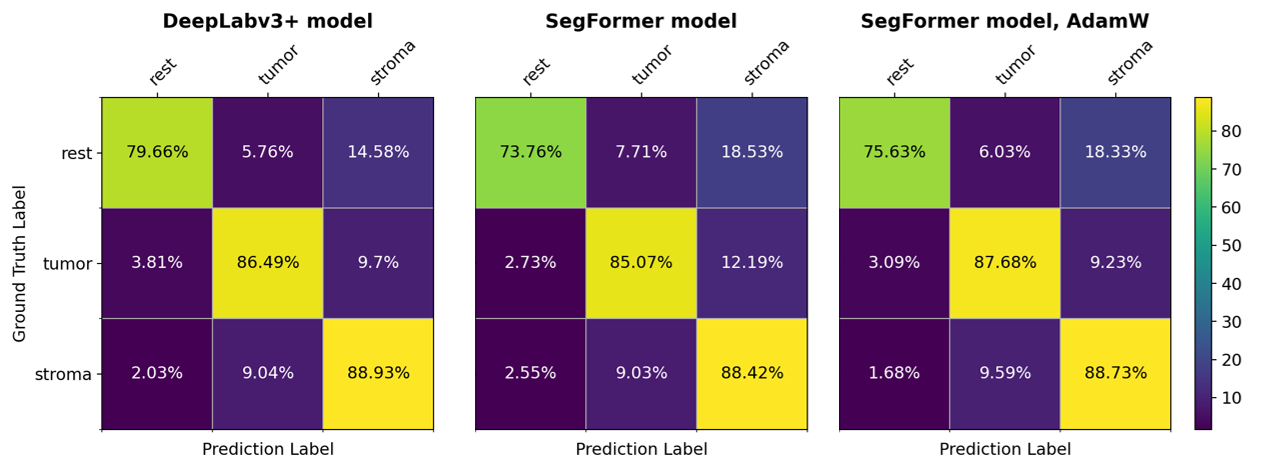
\includegraphics[width=\linewidth]{figures/tissue/conf_matrices.png}
    \caption{Confusion matrices on pixel level for DeepLabv3+, SegFormer and SegFormer with AdamW optimizer
    based on test set of 32 ROIs.}
    \label{fig:tissue_confusion}
\end{figure}

During the close investigation of test data, one slide (with the prefix TCGA-OL-A5RW-01Z-00-DX1)
was excluded from the test set due to an obvious image-mask mismatch. The overall
performance of the models, the number of parameters, and the resulting dice score after testing on 
32 test images can be found in Table~\ref*{tab:tissue_perform}.

The first thing that catches the eye is the severe runtime difference of
SegFormer-based methods compared to the DeepLabv3+ accompanied by doubled number of parameters.
None of the SegFormer approaches outperform the DeepLabv3+, but the performance
is comparable, which can be also observed in the confusion matrices in Figure~\ref*{fig:tissue_confusion}.

\begin{figure}[H]
    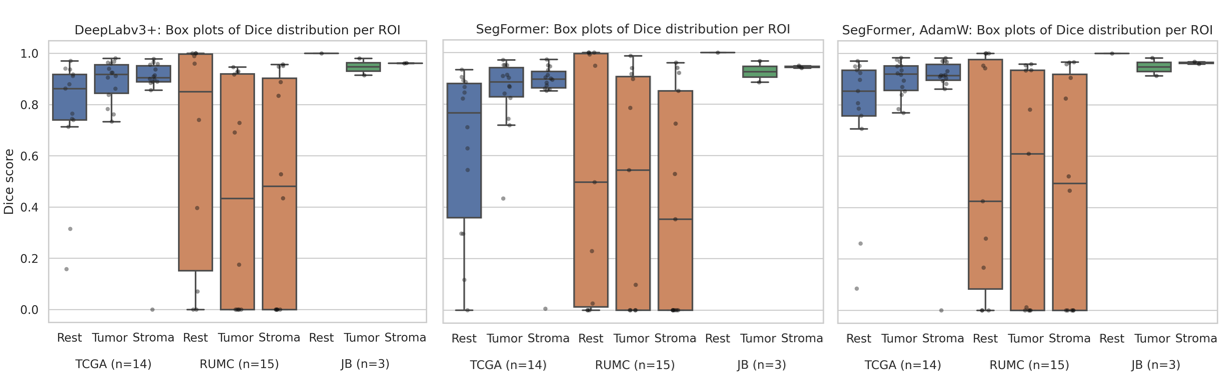
\includegraphics[width=\linewidth]{figures/tissue/dices.png}
    \caption{Boxplots of pixel wise calculated dice score across three datastes (TCGA-BRCA, RUMC, JB) and three segmentation labels.}
    \label{fig:tissue_dice_boxplots}
\end{figure} 

Both SegFormer-based methods show difficulty correctly segmenting rest regions, whereas
SegFormer AdamW slightly outperforms DeepLabv3+ in the number of true positive detected tumor pixels.
As previously mentioned, the dataset originates from three medical
institutions which make it reasonable to characterize the performance separately.
The boxplots in Figure~\ref*{fig:tissue_dice_boxplots} indicate that the performance of
the DeepLabv3+ and SegFormer AdamW models in TCGA-BRCA and JB groups are fairly invariant.
Whereas the RUMC group accounts not only for the lower performance of SegFormer-based methods
in segmenting rest regions but also for an improvement of tumor region segmentation by SegFormer AdamW
model both observed in Figure~\ref*{fig:tissue_confusion}.

The additional specialty that Figure~\ref*{fig:tissue_dice_boxplots} brings to light is
the considerable number of RUMC ROIs that have been evaluated with dice scores close to
zero across all models. Due to the nature of the Dice score, those can be originated from
significant numbers of either false positives, false negatives, or both.
According to the boxplots of precision and recall in Figure~\ref*{fig:tissue_pr_r_boxplots}
the precision across all models has more close zero values that indicate more frequent
false positives. There are clear examples, such as Figure~\ref*{fig:TC_S01_P000159},
where the ground truth includes exclusively rest but all trained models provide multiple class predicitons.
Even though there are also opposite examples of regions that were solely annotated as rest and predicted as
such (which then lead to occasional dice, precision, and recall equal to one),
the issue of false positives, in this case, might be solved only by finding a
better dataset split. 

A close look at the prediction also revealed that at some cases dice scores might suffer due to some inaccuracies
in the annotations. Figure~\ref*{fig:TCGA-GM-A2DF} showcases that all models were
penalized for detecting a rest region inside of the tumor, which was probably learned
with some dependency to the presence of white space, which also present in the same slide
(the bubles in the lower part of the image) and was annotated as rest.

Nonetheless, there are positive segmentation results present, such as JB ROIs depicted in
Figure~\ref*{fig:s_250B_1} and~\ref*{fig:s_250B_2} where the performance of SegFormer AdamW
is either very close or slightly better then DeepLabv3+ or like in Figure~\ref*{fig:TCGA-EW-A1P4}
where SegFormer AdamW is significantly more accurate. Yet while 
the SegFormer AdamW model remains promising, due to overall better performance and
runtime, this thesis will use the DeepLabv3+ model for further inferences and analysis.

\begin{figure}[H]
    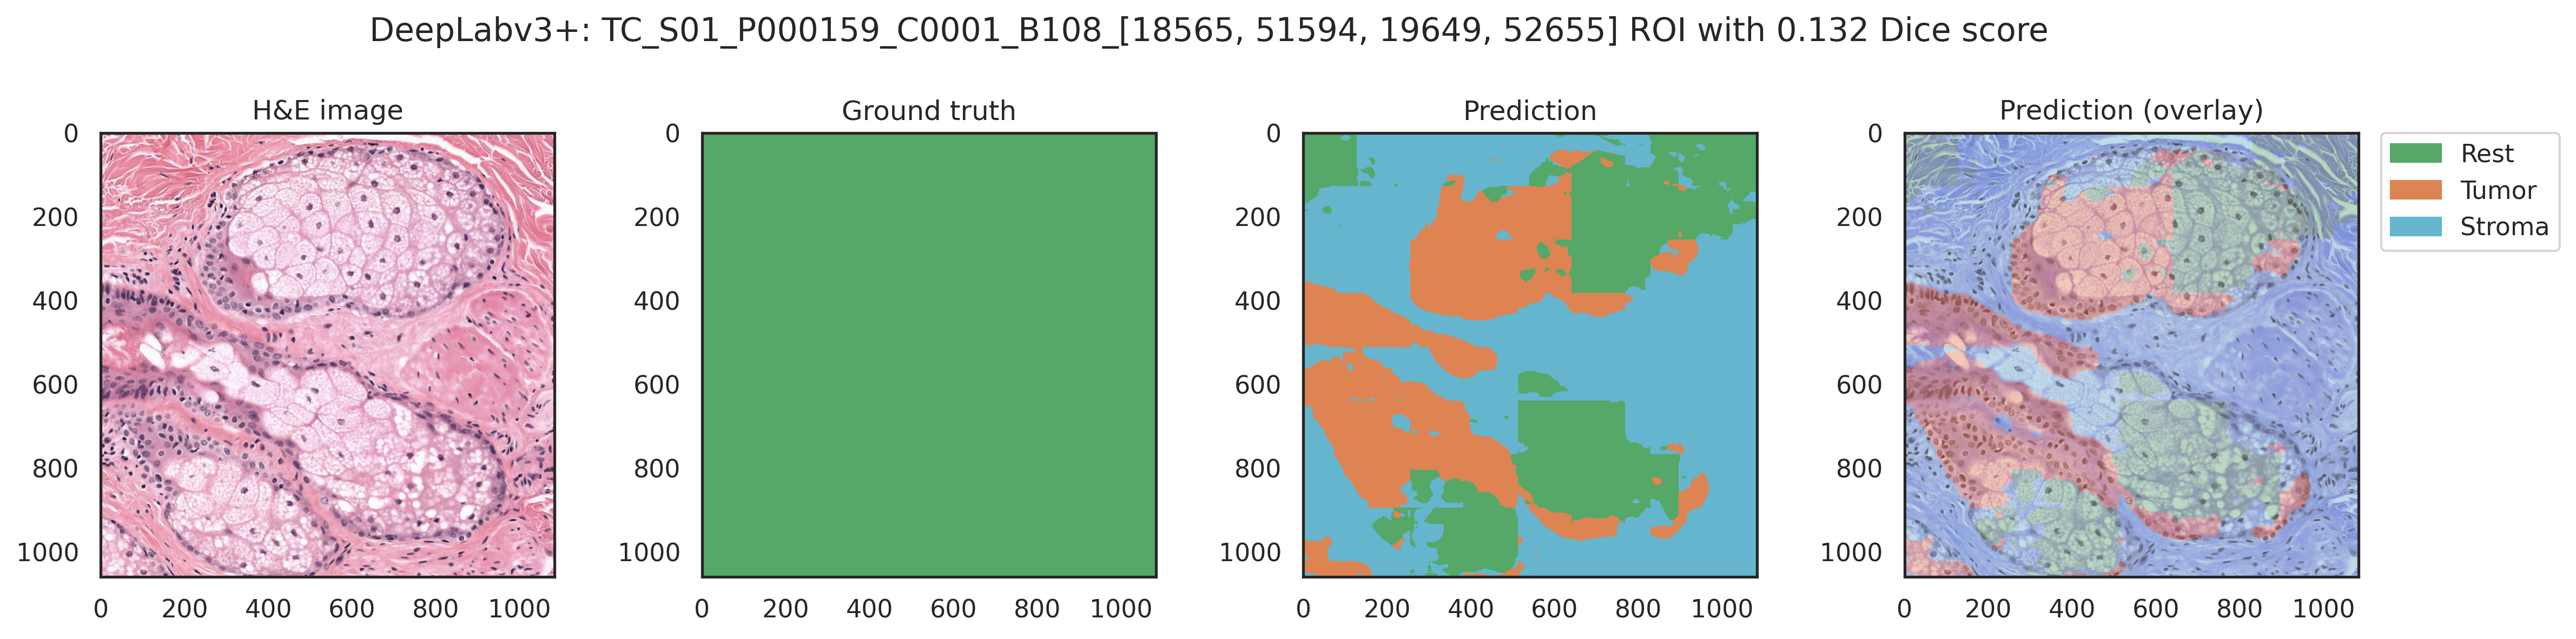
\includegraphics[width=\linewidth]{figures/tissue/deeplabv3+_dice_tc_TC_S01_P000159_C0001_B108_[18565,_51594,_19649,_52655]_check.png}
    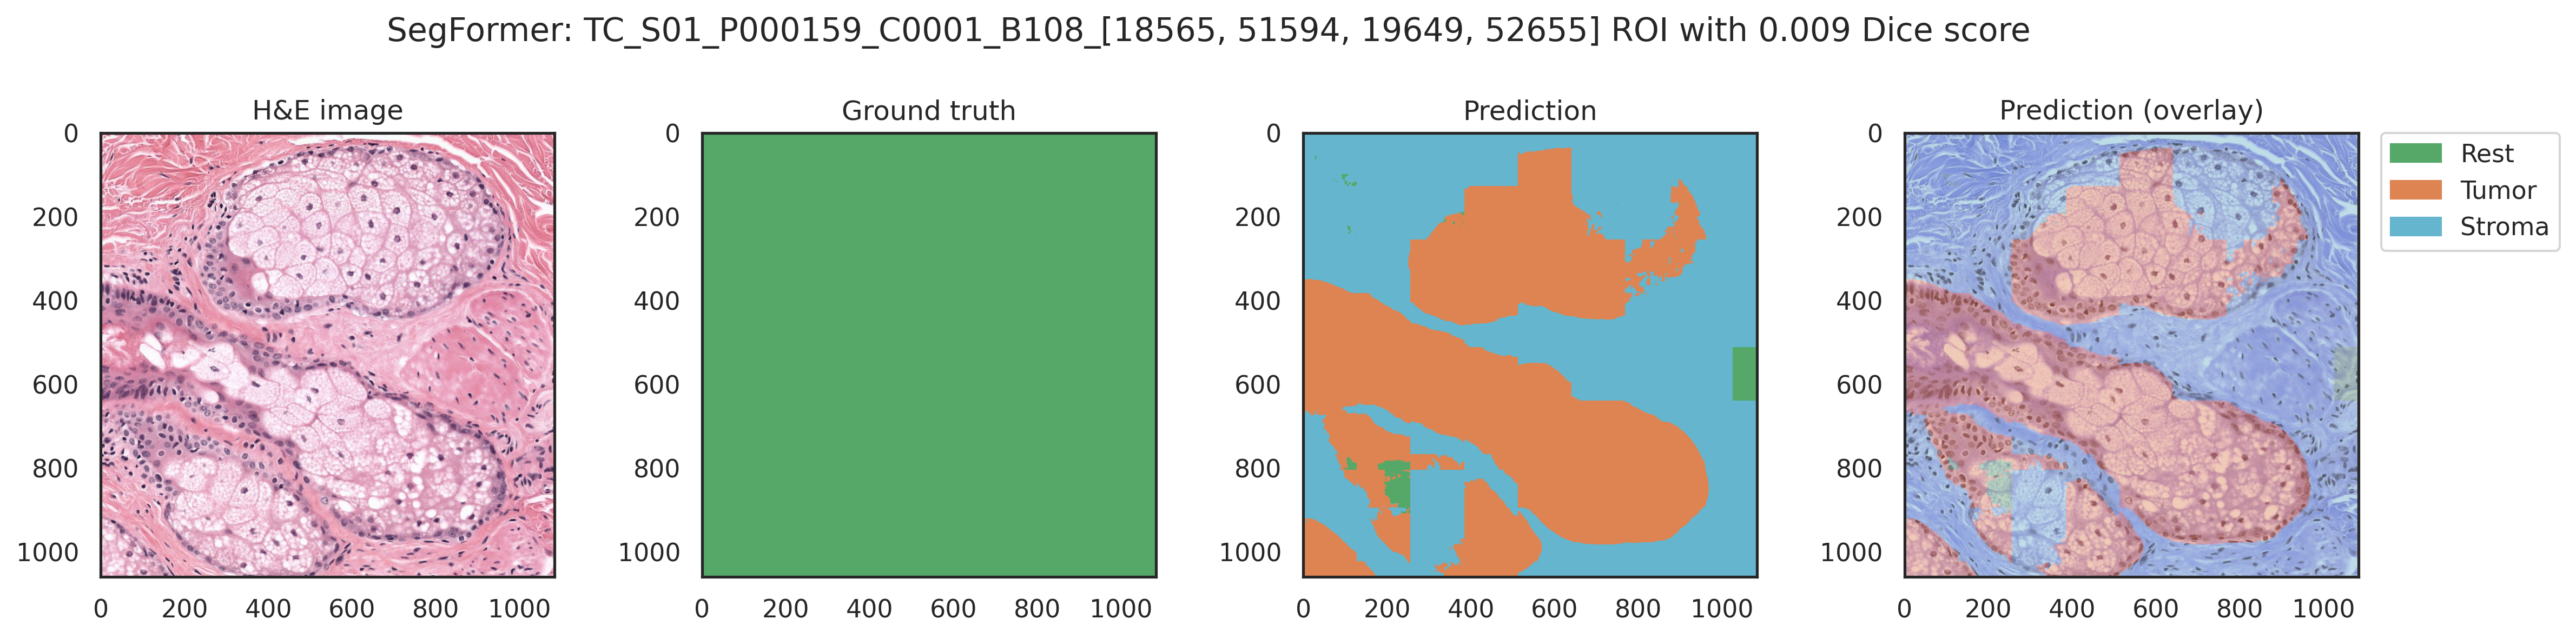
\includegraphics[width=\linewidth]{figures/tissue/segformer_dice_tc_TC_S01_P000159_C0001_B108_[18565,_51594,_19649,_52655]_check.png}
    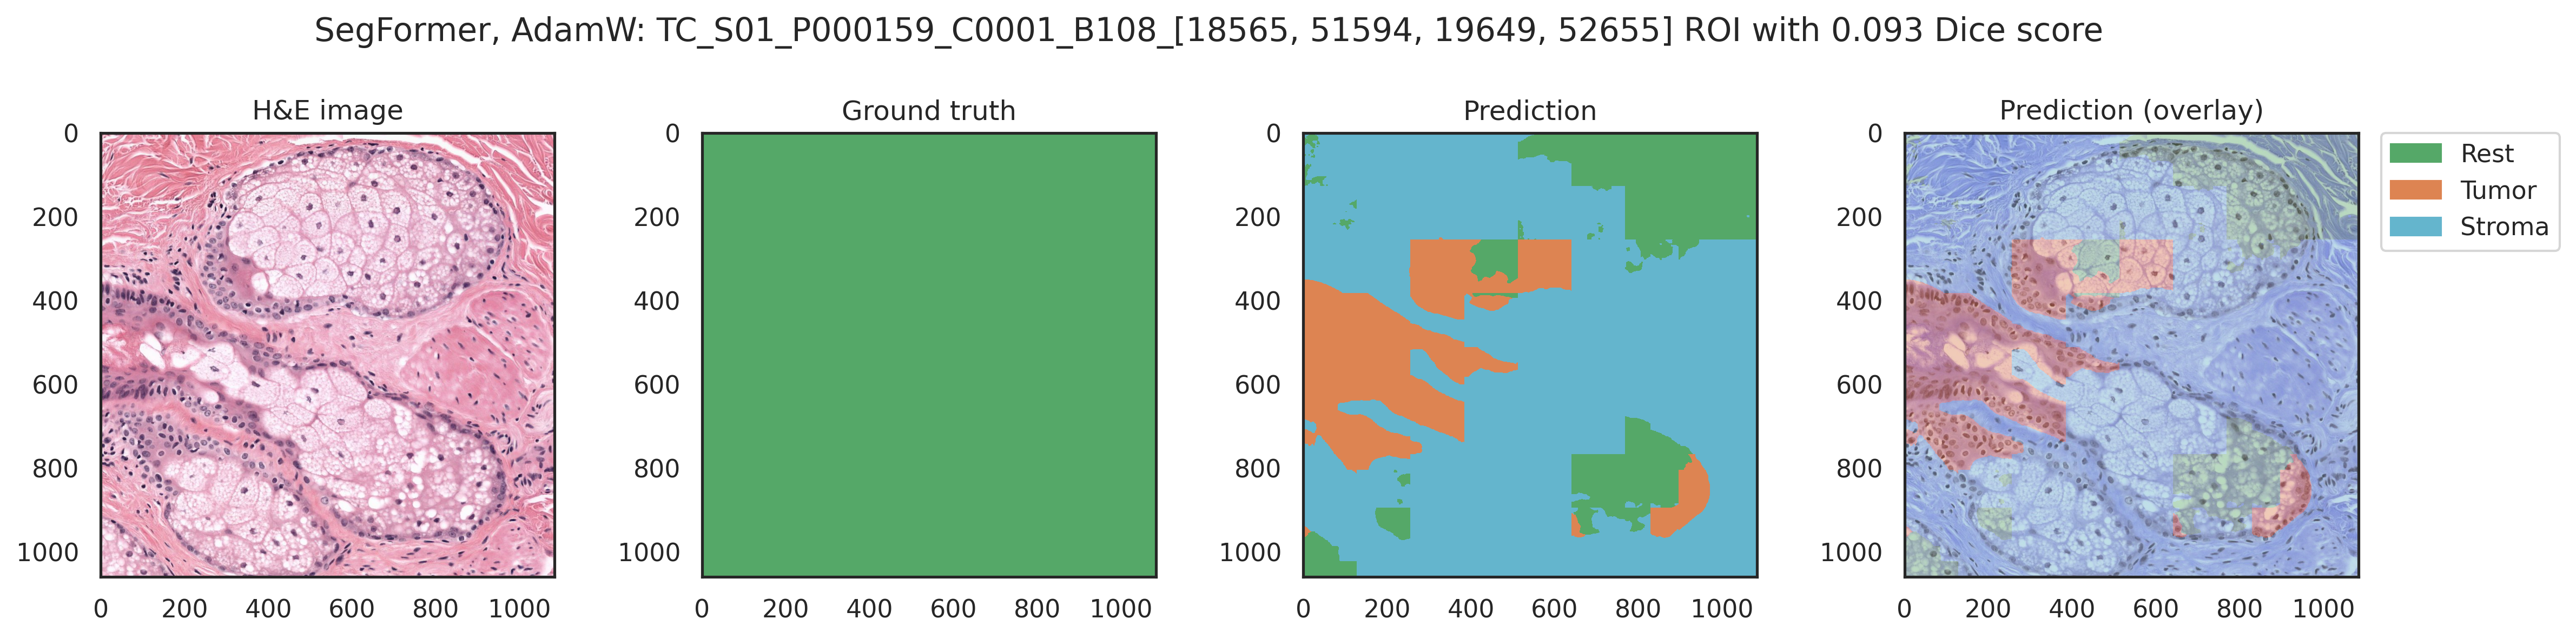
\includegraphics[width=\linewidth]{figures/tissue/segformer,_adamw_dice_tc_TC_S01_P000159_C0001_B108_[18565,_51594,_19649,_52655]_check.png}
    \caption{Example of rich false positive segmentation RUMC ROI that contributes to the cases of close zero dice scores.}
    \label{fig:TC_S01_P000159}
\end{figure}

\begin{figure}[H]
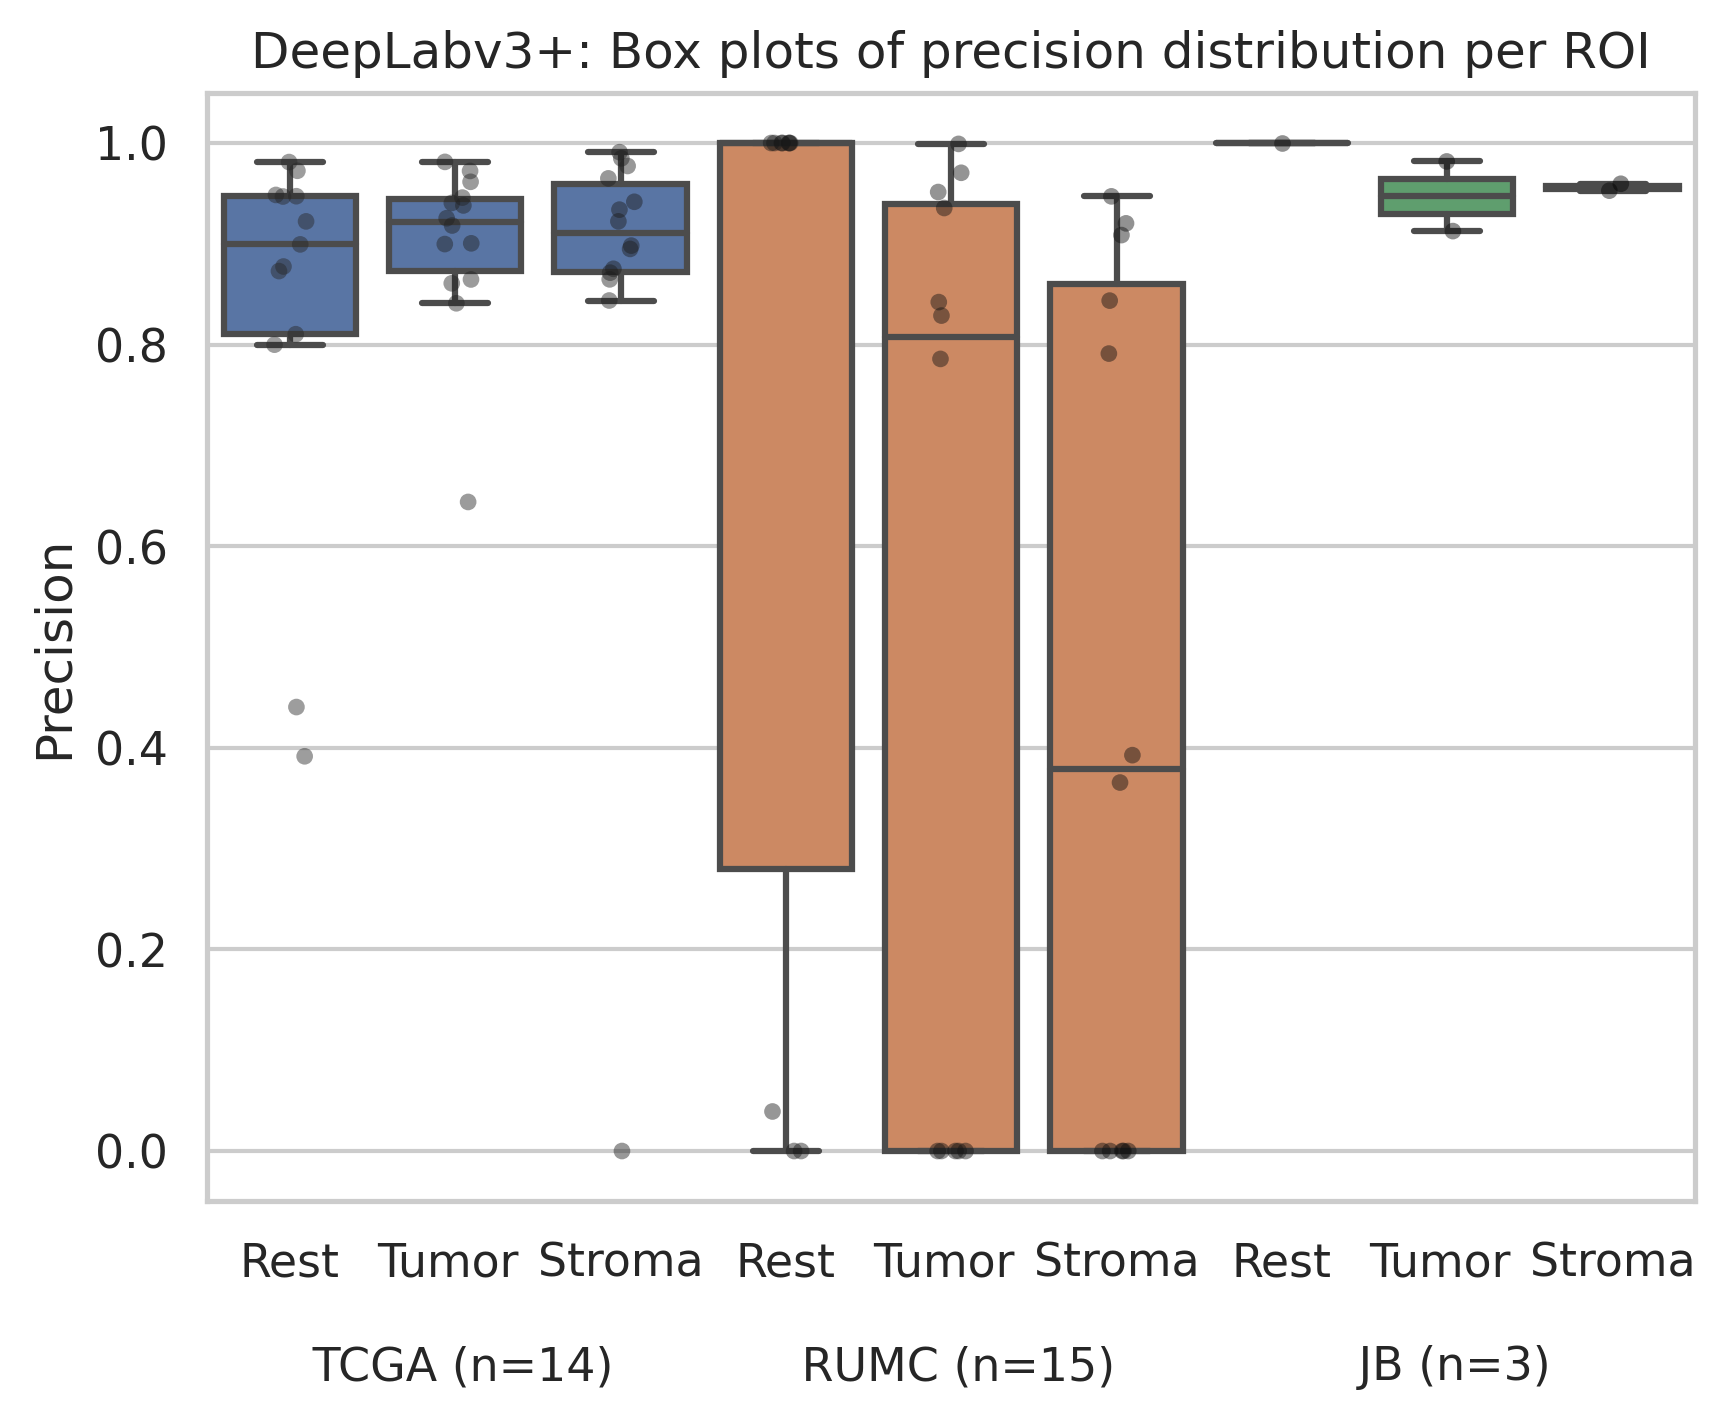
\includegraphics[width=.5\linewidth]{figures/tissue/deeplabv3+_prec_roi_wsirois.png}
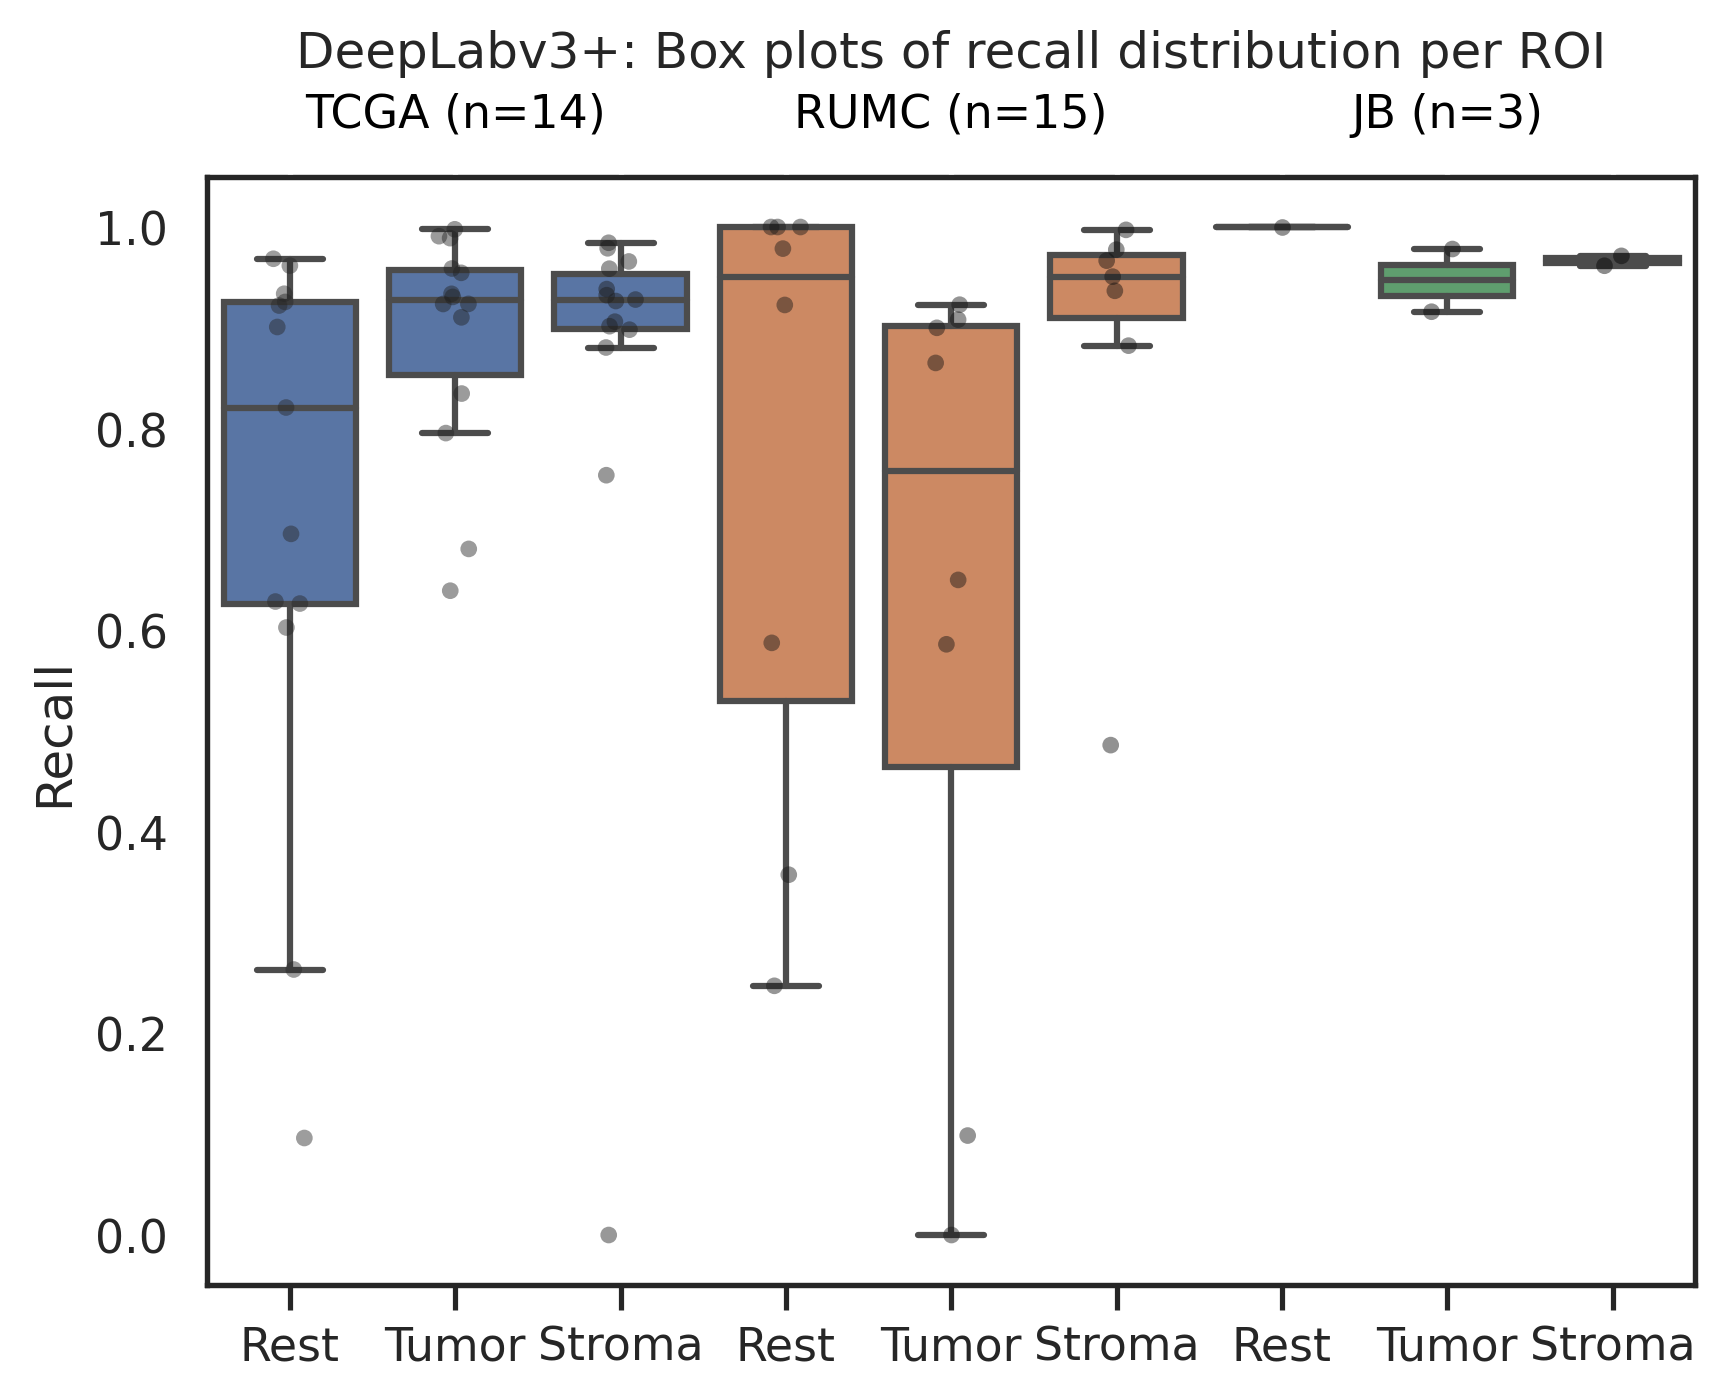
\includegraphics[width=.5\linewidth]{figures/tissue/deeplabv3+_recall_roi_wsirois.png}

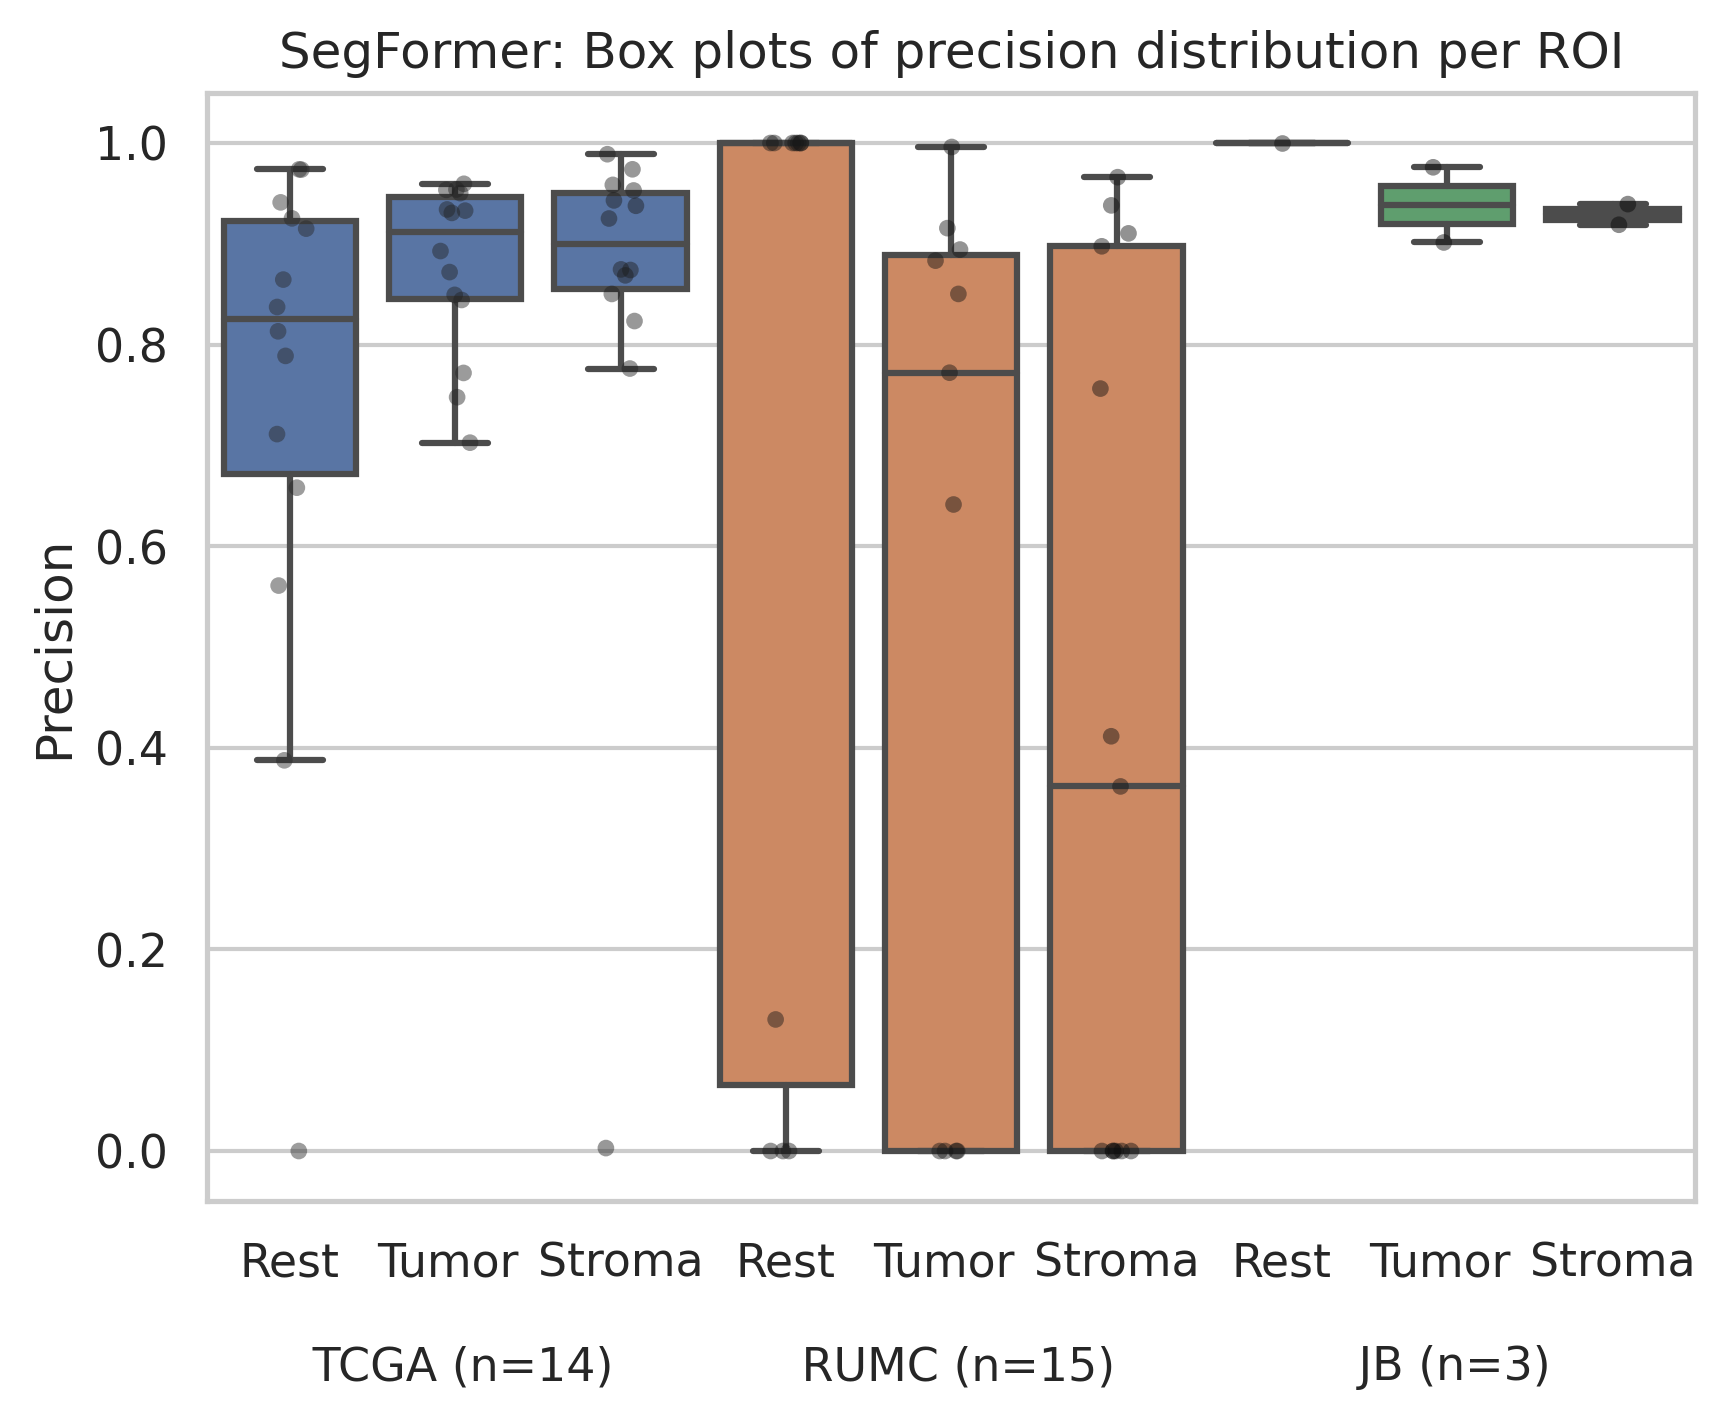
\includegraphics[width=.5\linewidth]{figures/tissue/segformer_prec_roi_wsirois.png}
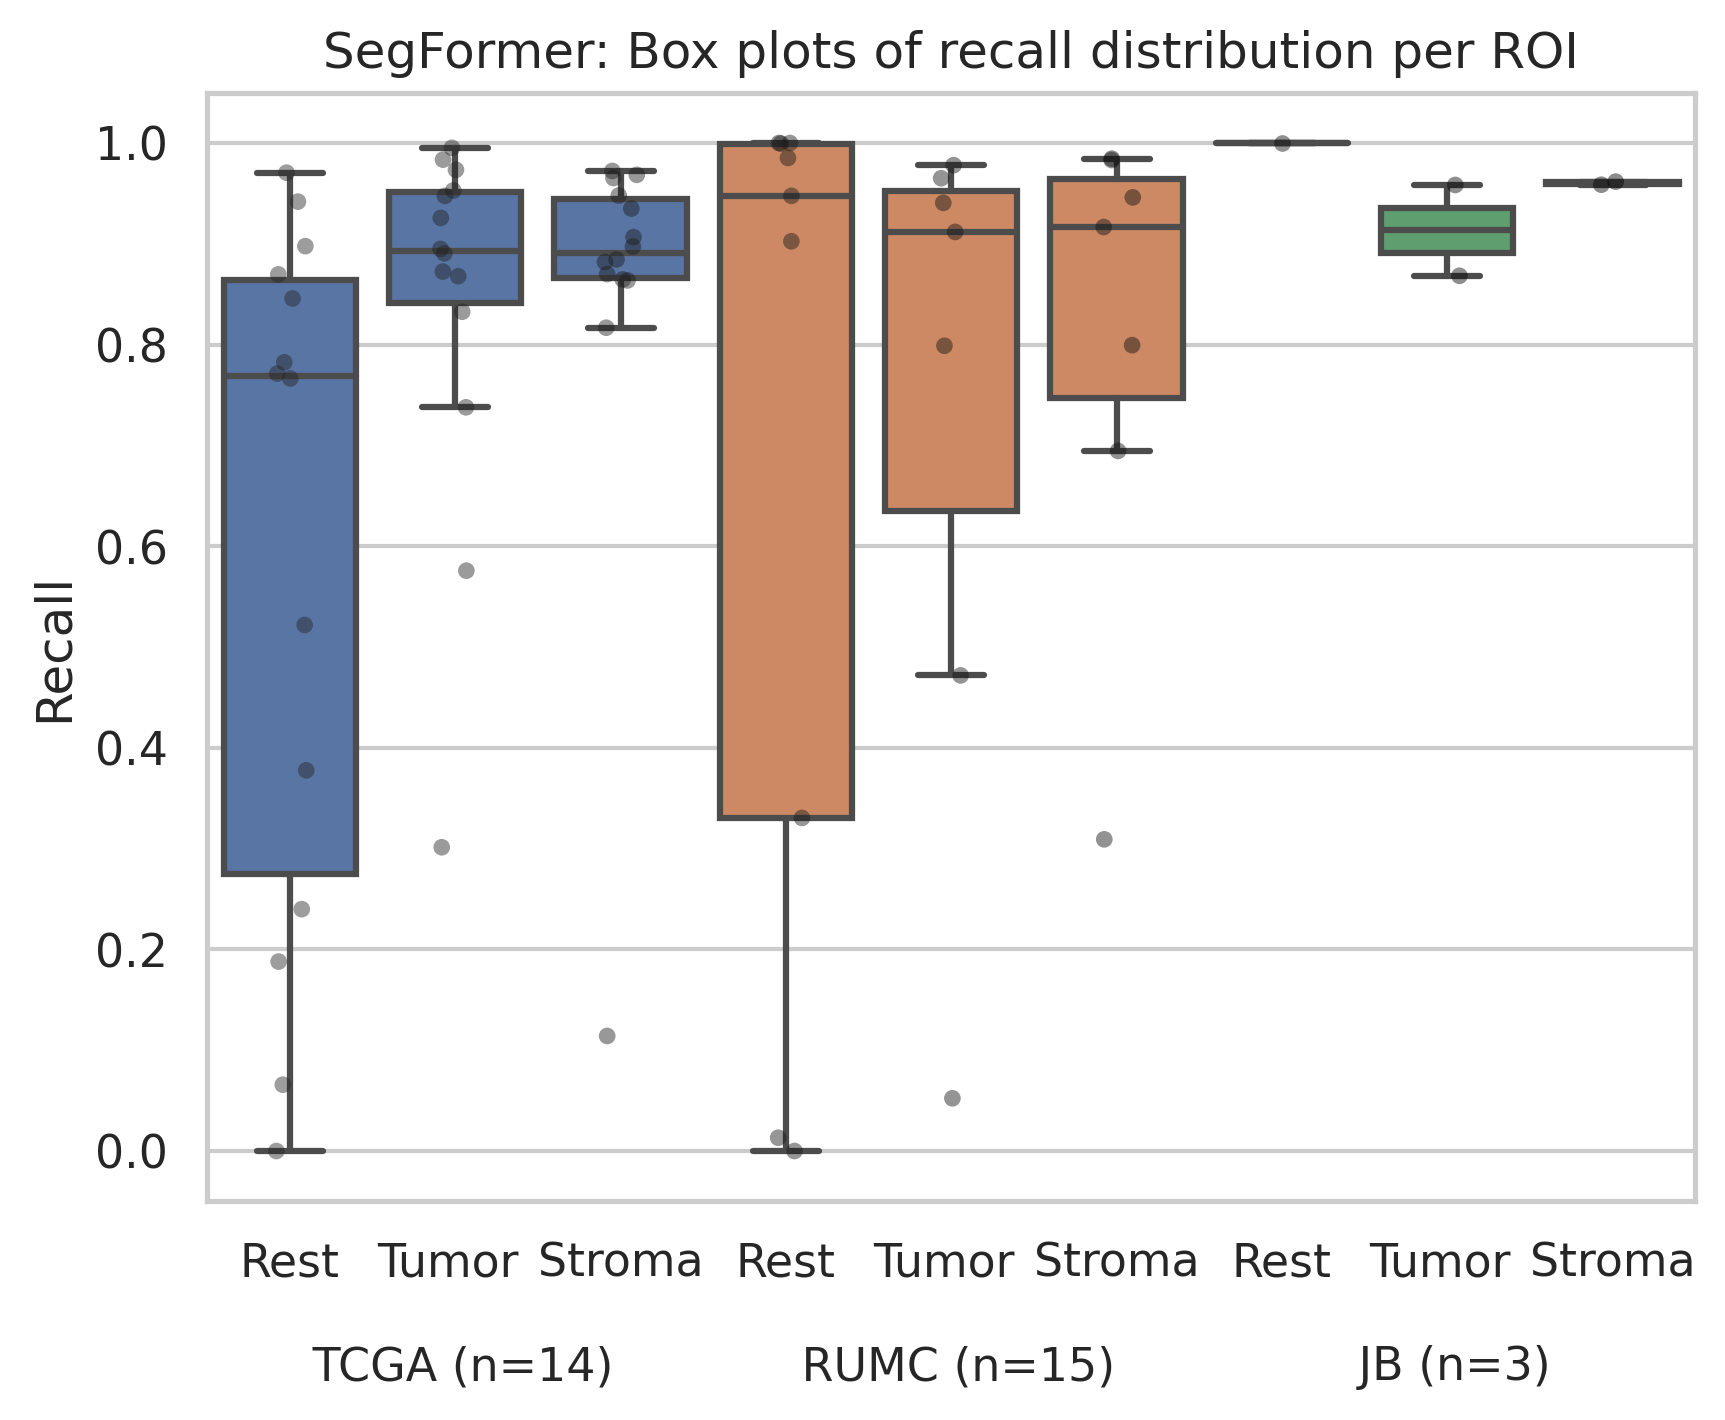
\includegraphics[width=.5\linewidth]{figures/tissue/segformer_recall_roi_wsirois.png}

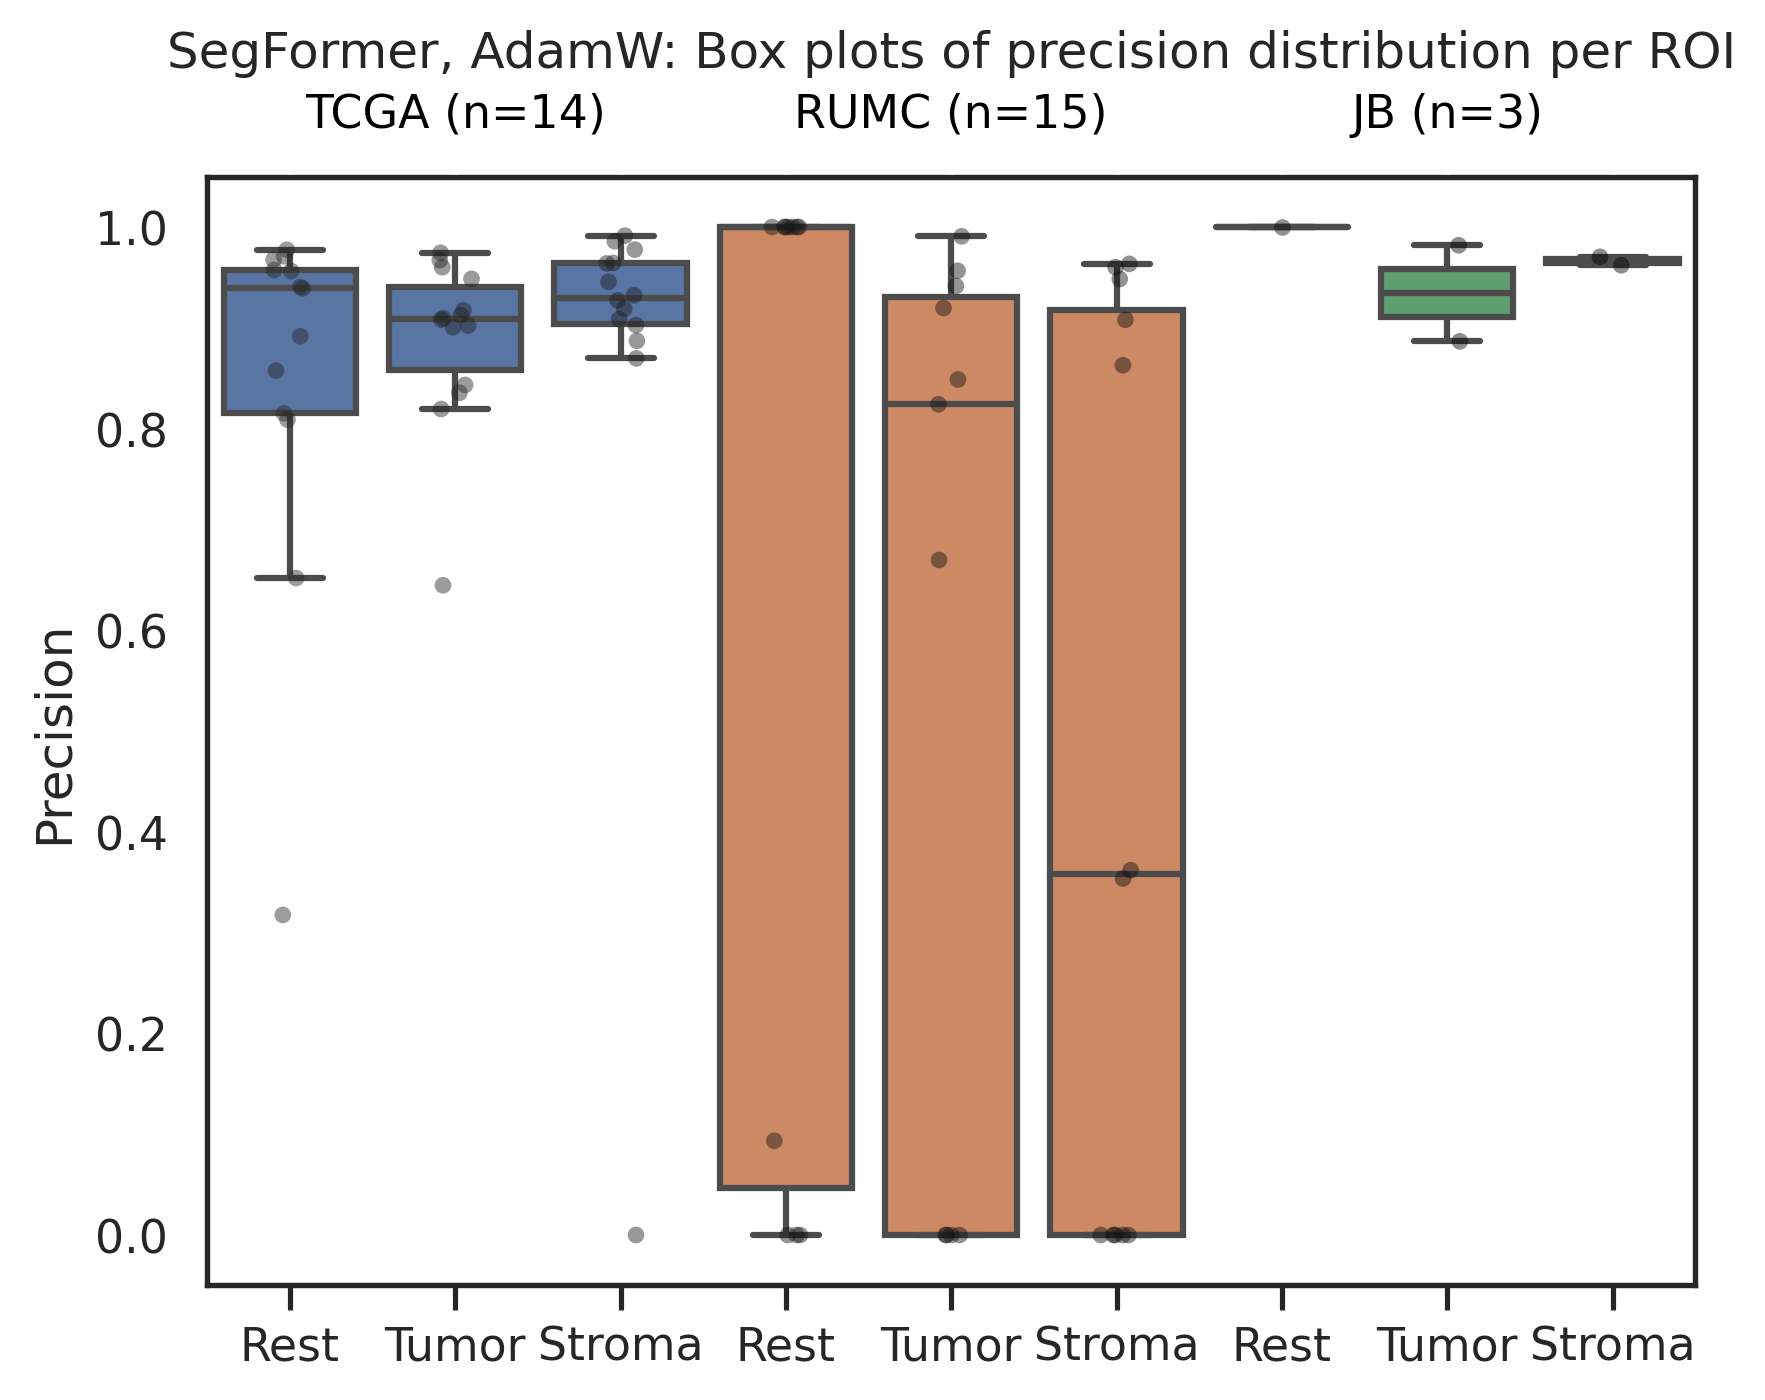
\includegraphics[width=.5\linewidth]{figures/tissue/segformer,_adamw_prec_roi_wsirois.png}
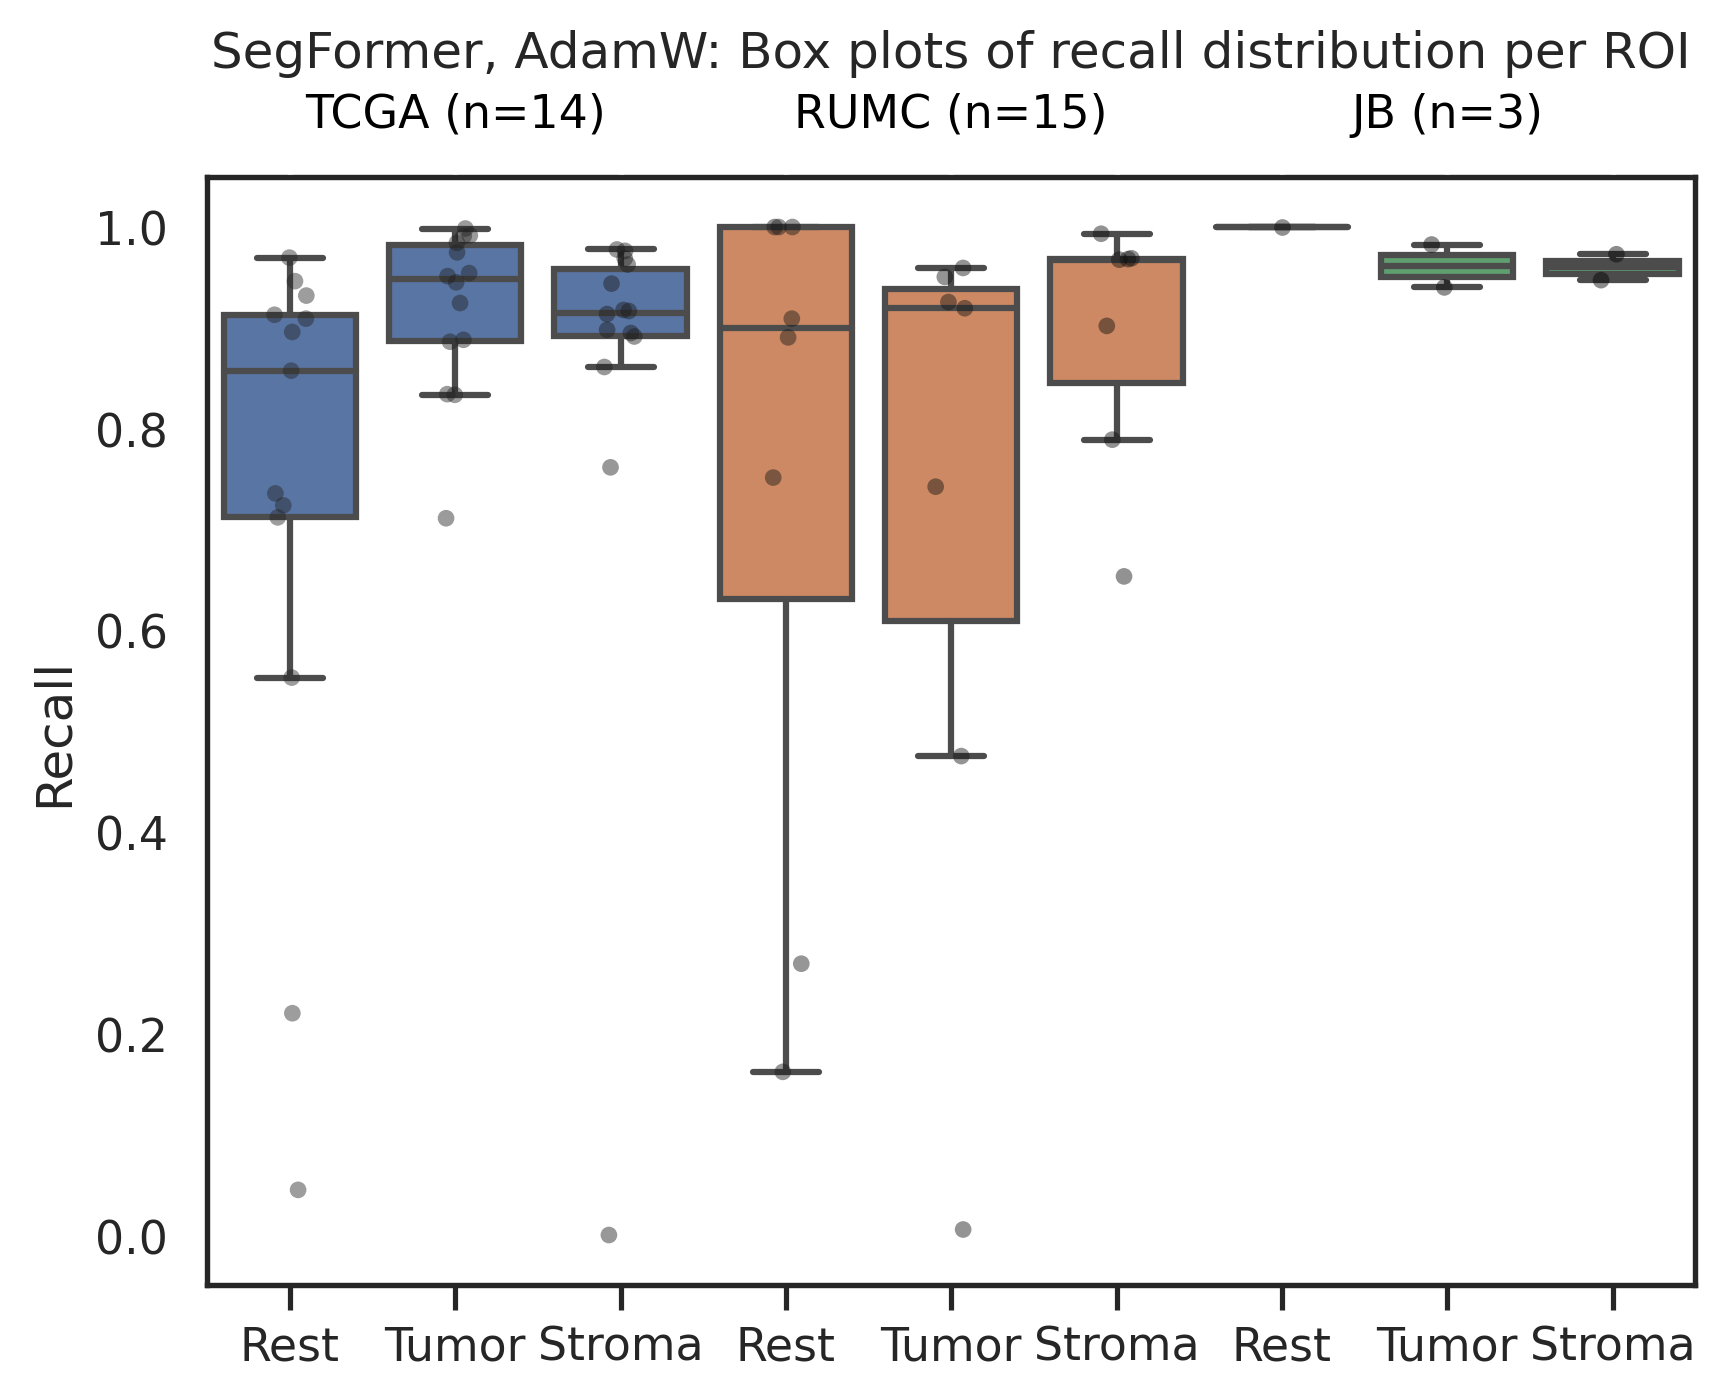
\includegraphics[width=.5\linewidth]{figures/tissue/segformer,_adamw_recall_roi_wsirois.png}
\caption{Boxplots of pixel wise calculated precision and recall across three datastes (TCGA-BRCA, RUMC, JB) and three segmentation labels.}
\label{fig:tissue_pr_r_boxplots}
\end{figure}

\begin{figure}[H]
    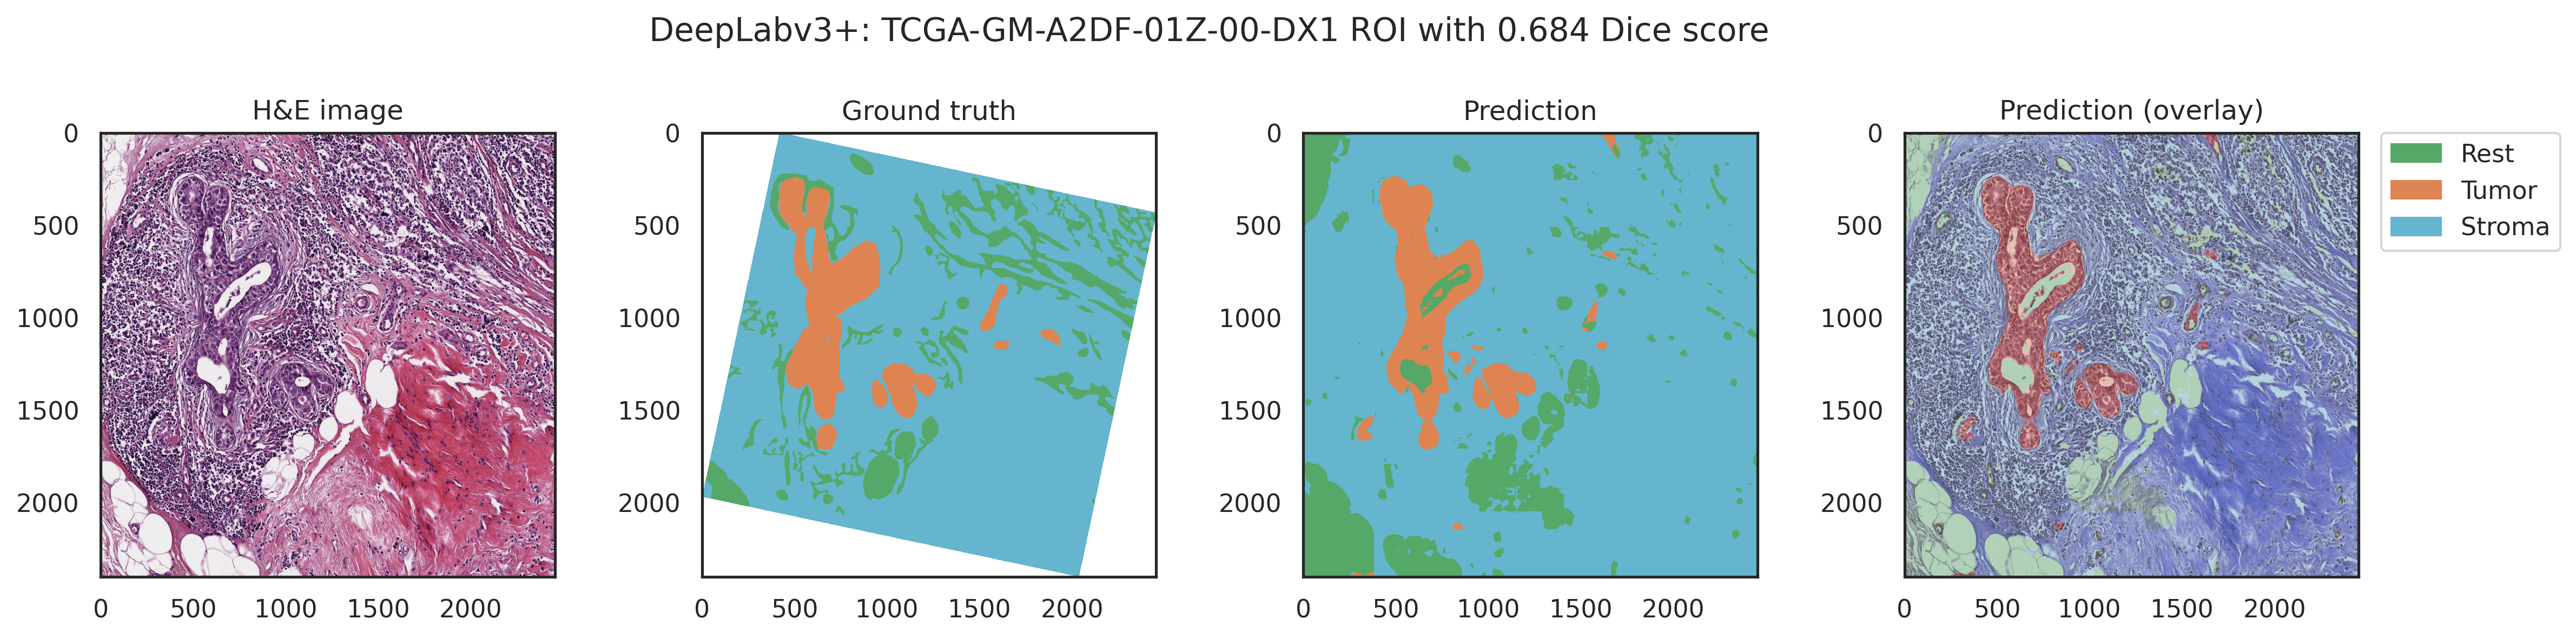
\includegraphics[width=\linewidth]{figures/tissue/deeplabv3+_dice_tcga_TCGA-GM-A2DF-01Z-00-DX1CD0BE6D7-2DB3-4193-84CC-F9BE7BF18CC2_[25322,_21890,_27778,_24293]_check.png}
    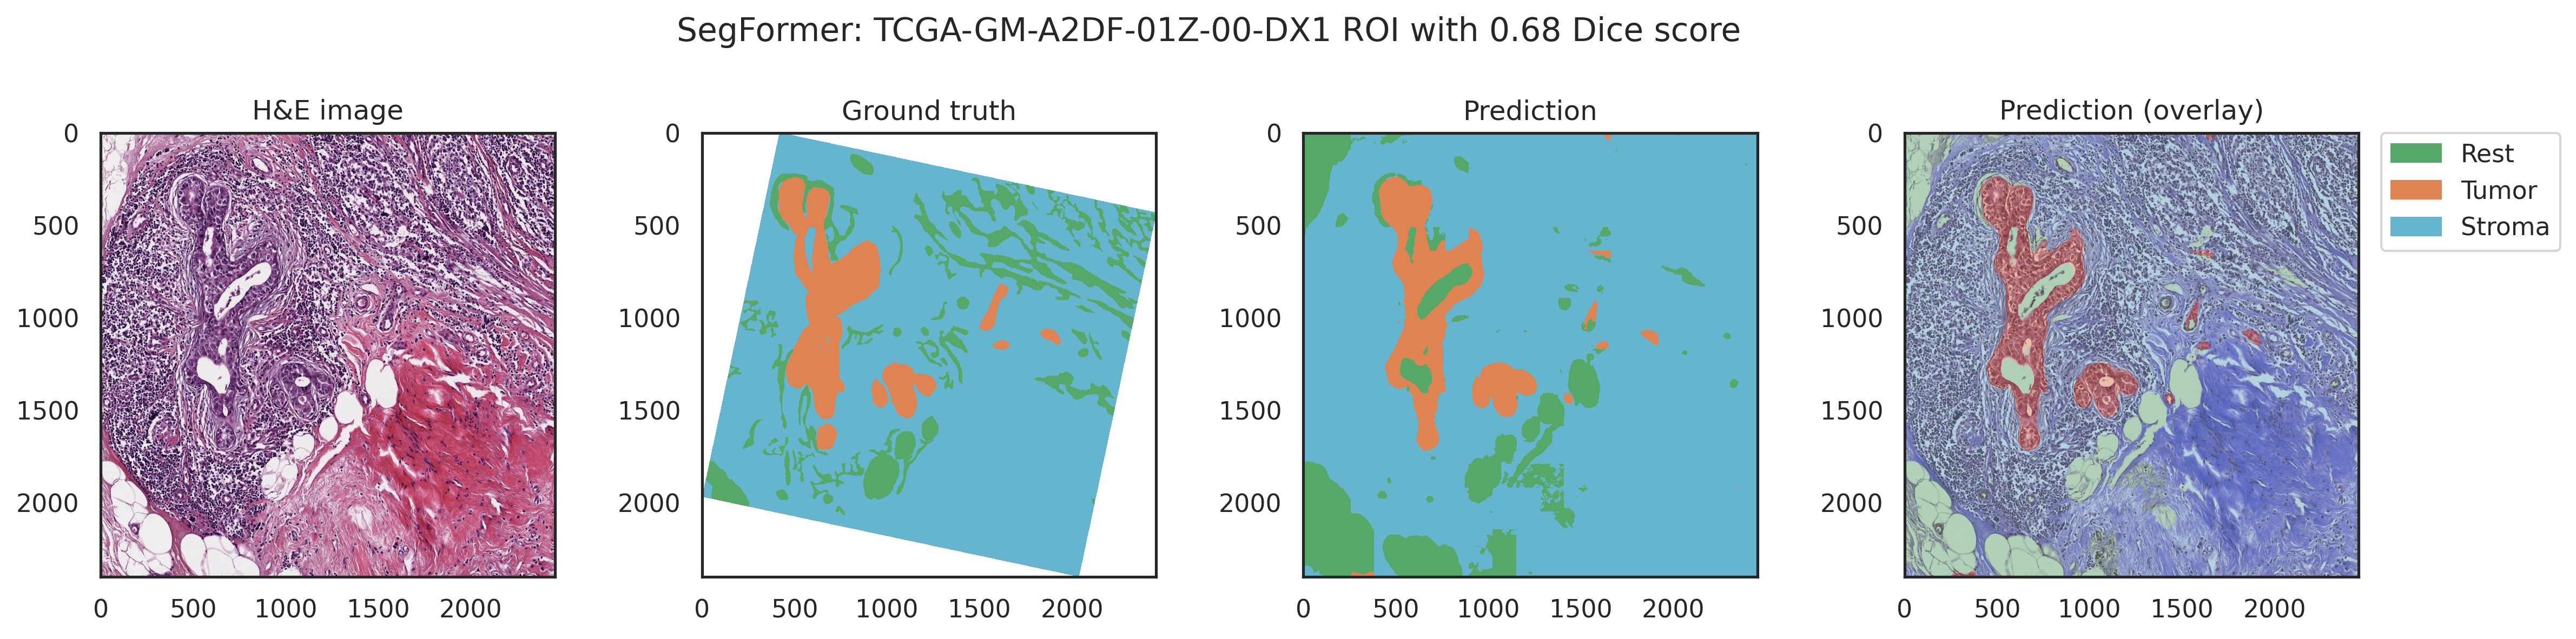
\includegraphics[width=\linewidth]{figures/tissue/segformer_dice_tcga_TCGA-GM-A2DF-01Z-00-DX1CD0BE6D7-2DB3-4193-84CC-F9BE7BF18CC2_[25322,_21890,_27778,_24293]_check.png}
    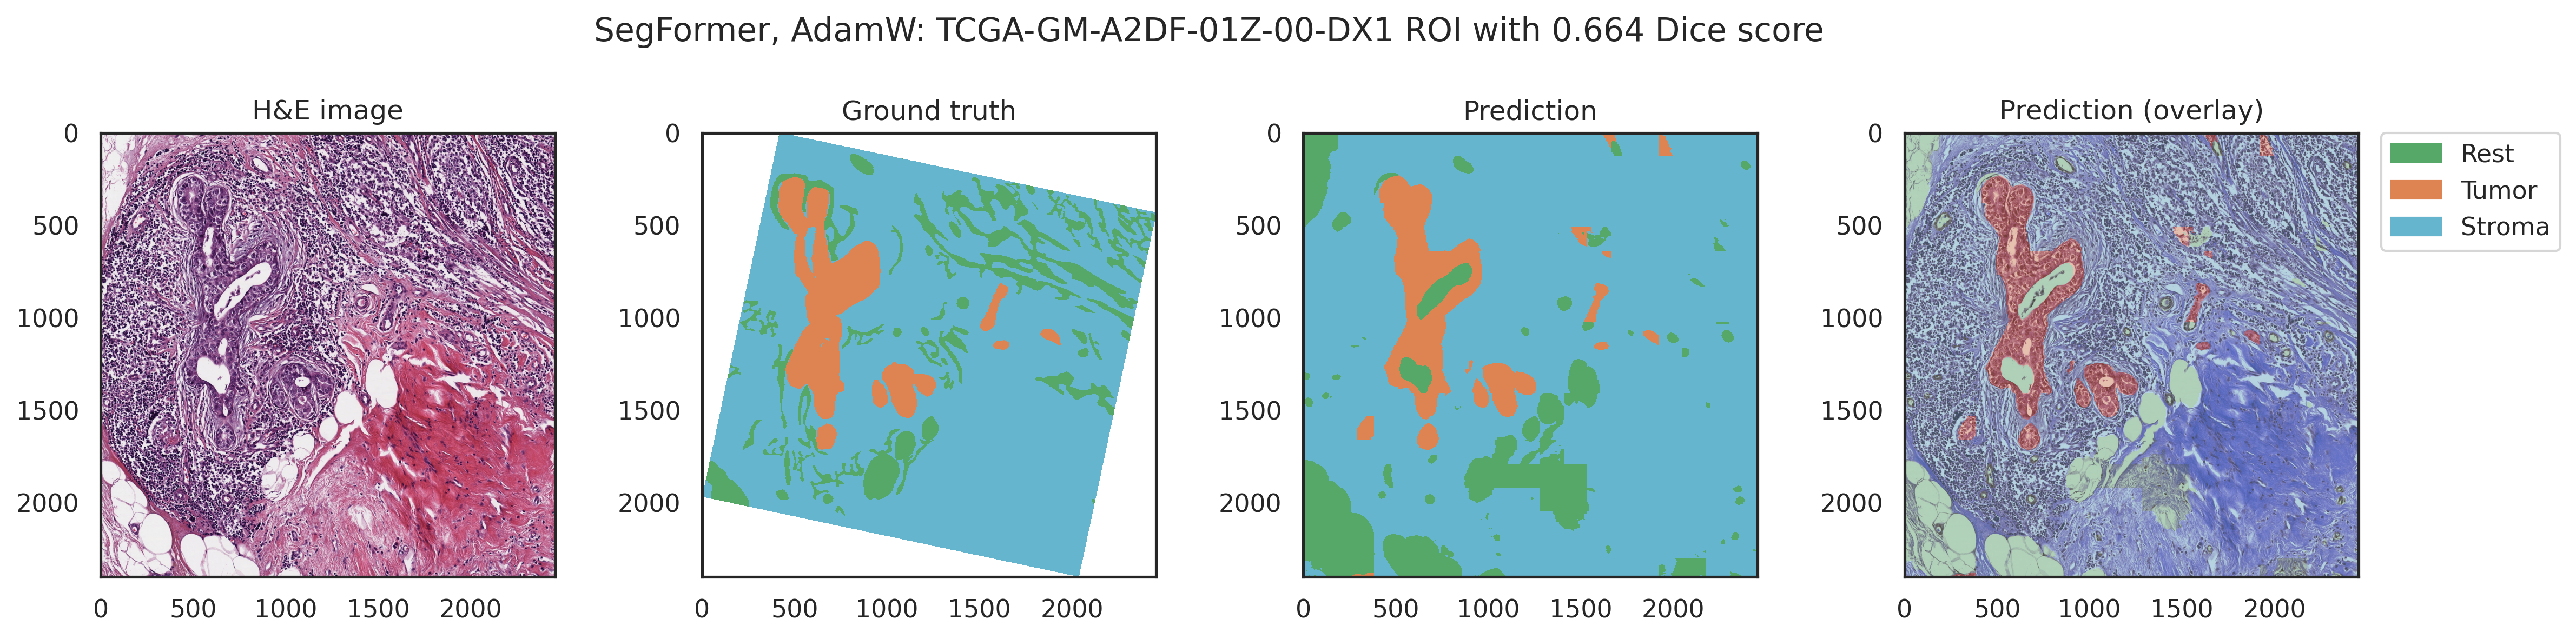
\includegraphics[width=\linewidth]{figures/tissue/segformer,_adamw_dice_tcga_TCGA-GM-A2DF-01Z-00-DX1CD0BE6D7-2DB3-4193-84CC-F9BE7BF18CC2_[25322,_21890,_27778,_24293]_check.png}
    
    \caption{Example of a slightly devalued dice score due to some annotation inaccuracies.}
    \label{fig:TCGA-GM-A2DF}
\end{figure}
    

\begin{figure}[H]
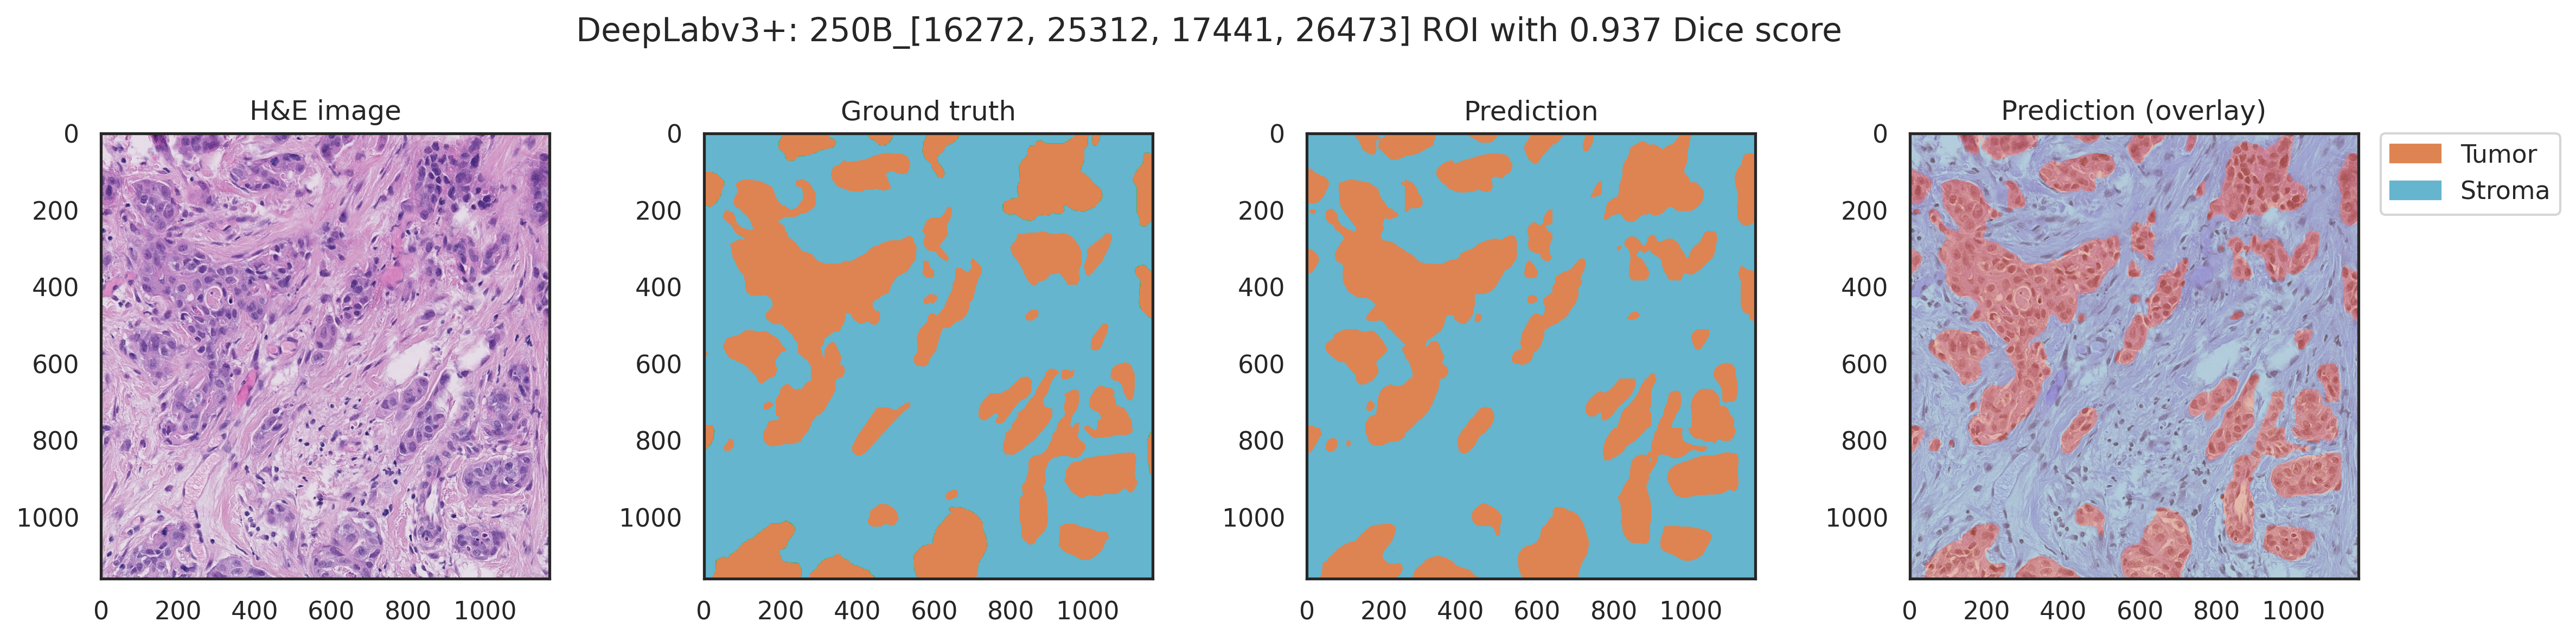
\includegraphics[width=\linewidth]{figures/tissue/deeplabv3+_dice_s_250B_[16272,_25312,_17441,_26473]_check.png}
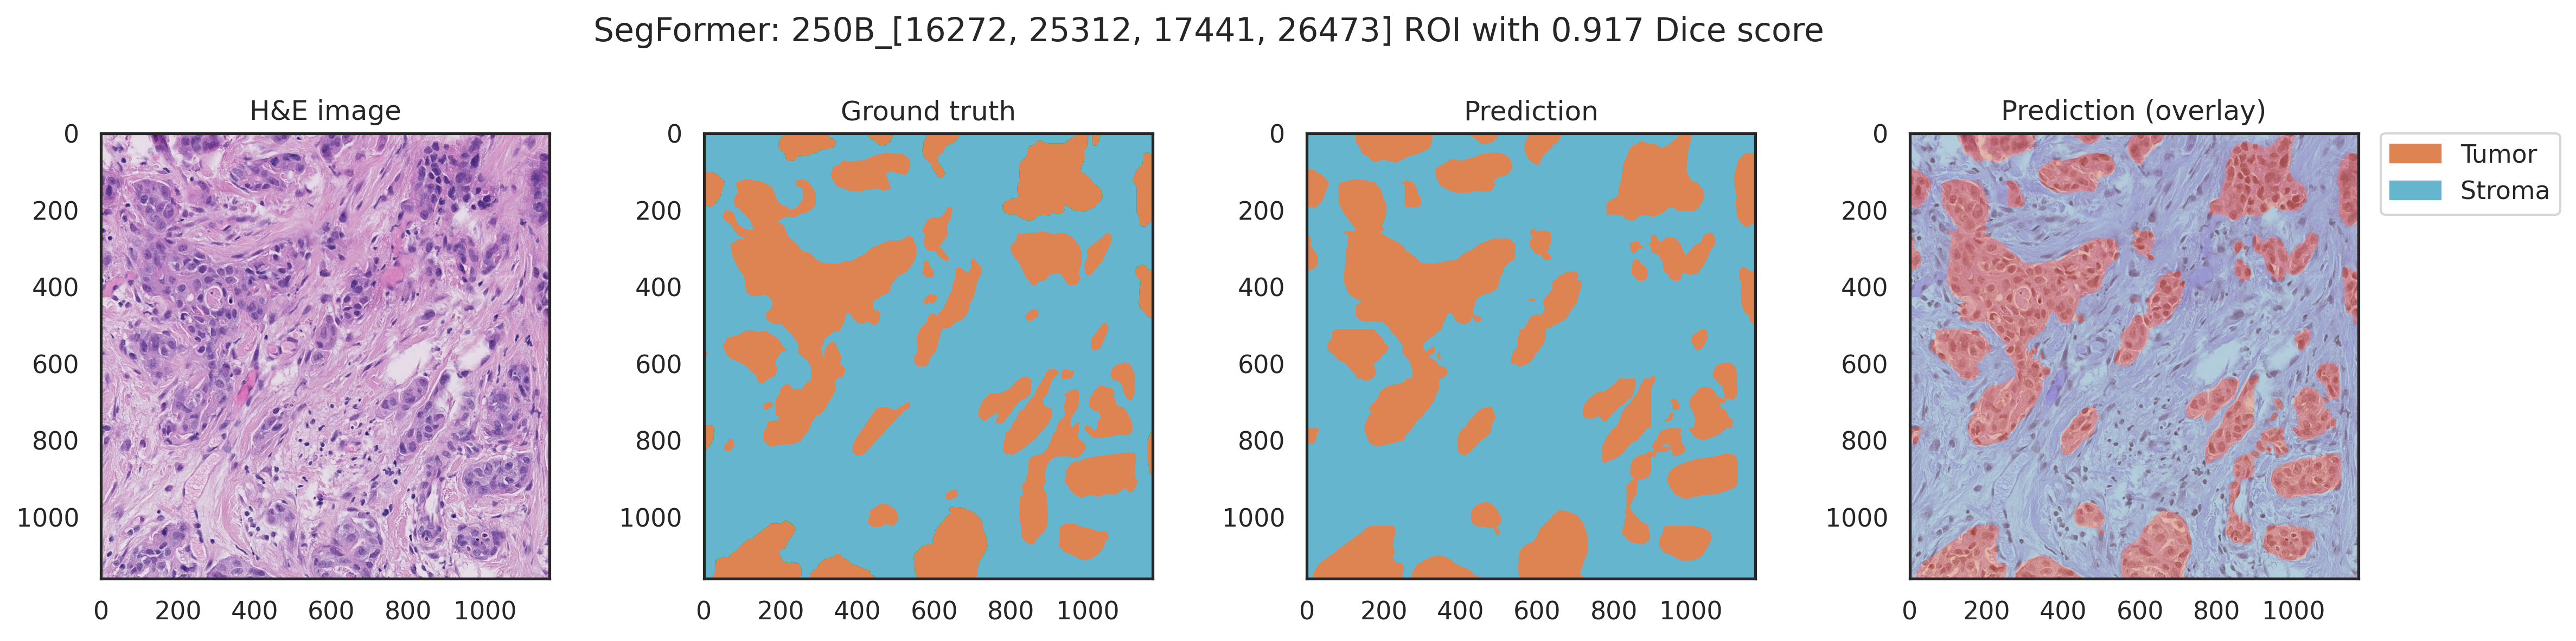
\includegraphics[width=\linewidth]{figures/tissue/segformer_dice_s_250B_[16272,_25312,_17441,_26473]_check.png}
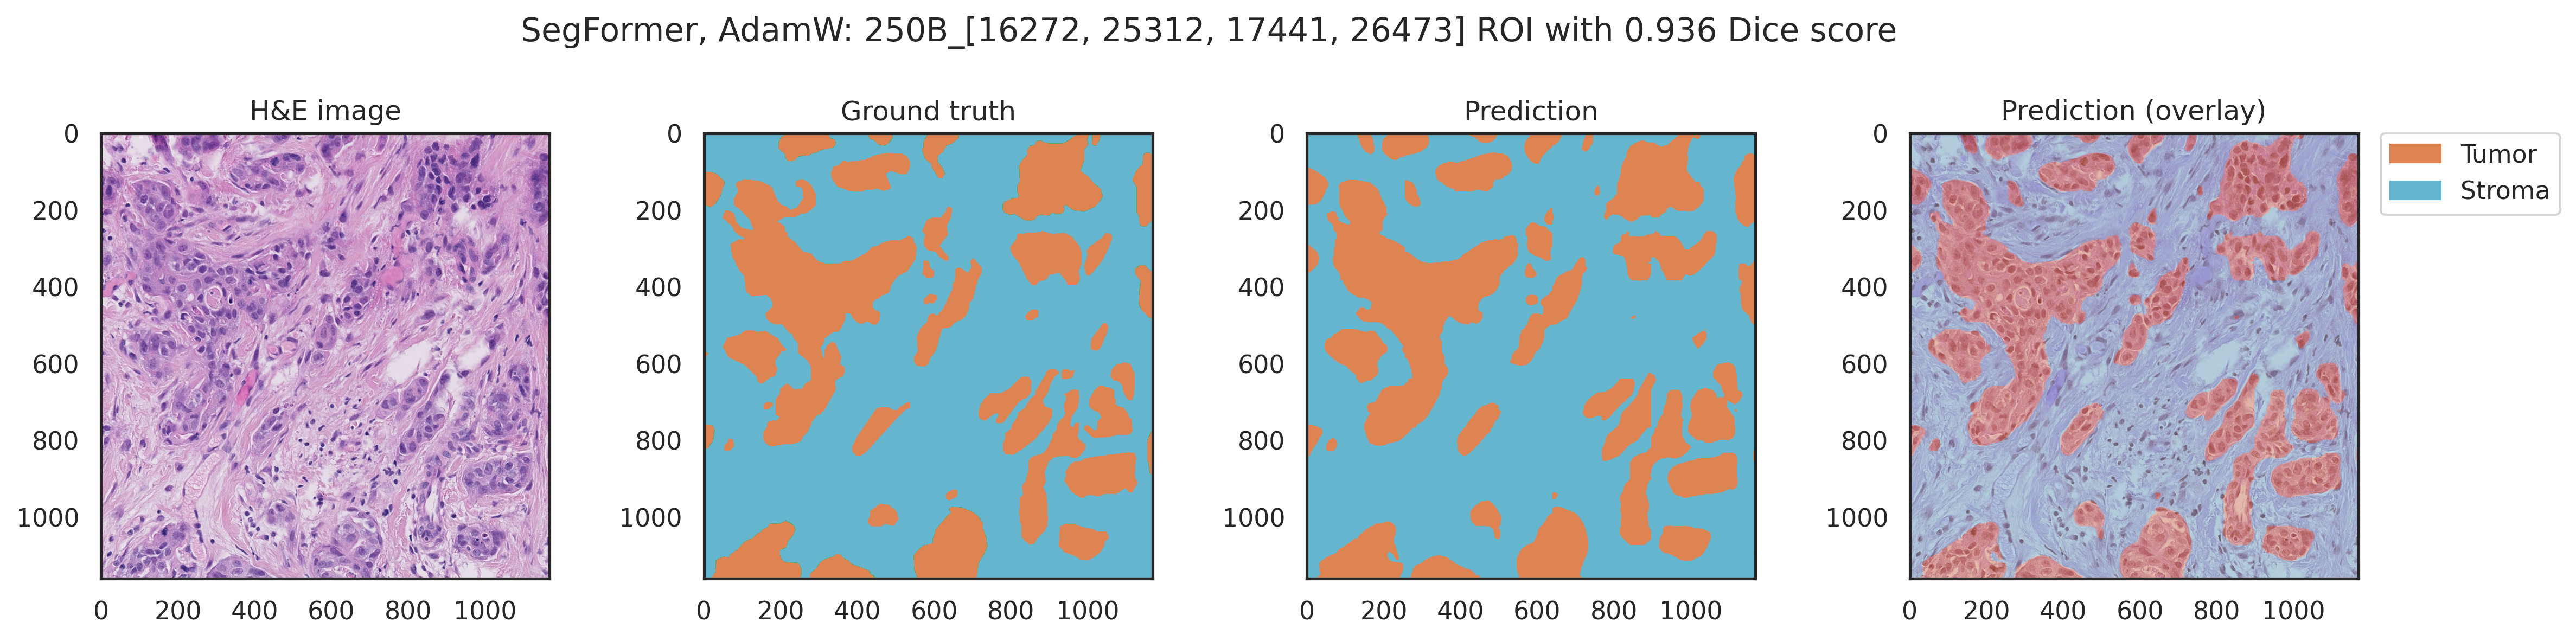
\includegraphics[width=\linewidth]{figures/tissue/segformer,_adamw_dice_s_250B_[16272,_25312,_17441,_26473]_check.png}

\caption{JB ROI segmentation result.}
\label{fig:s_250B_1}
\end{figure}

\begin{figure}[H]
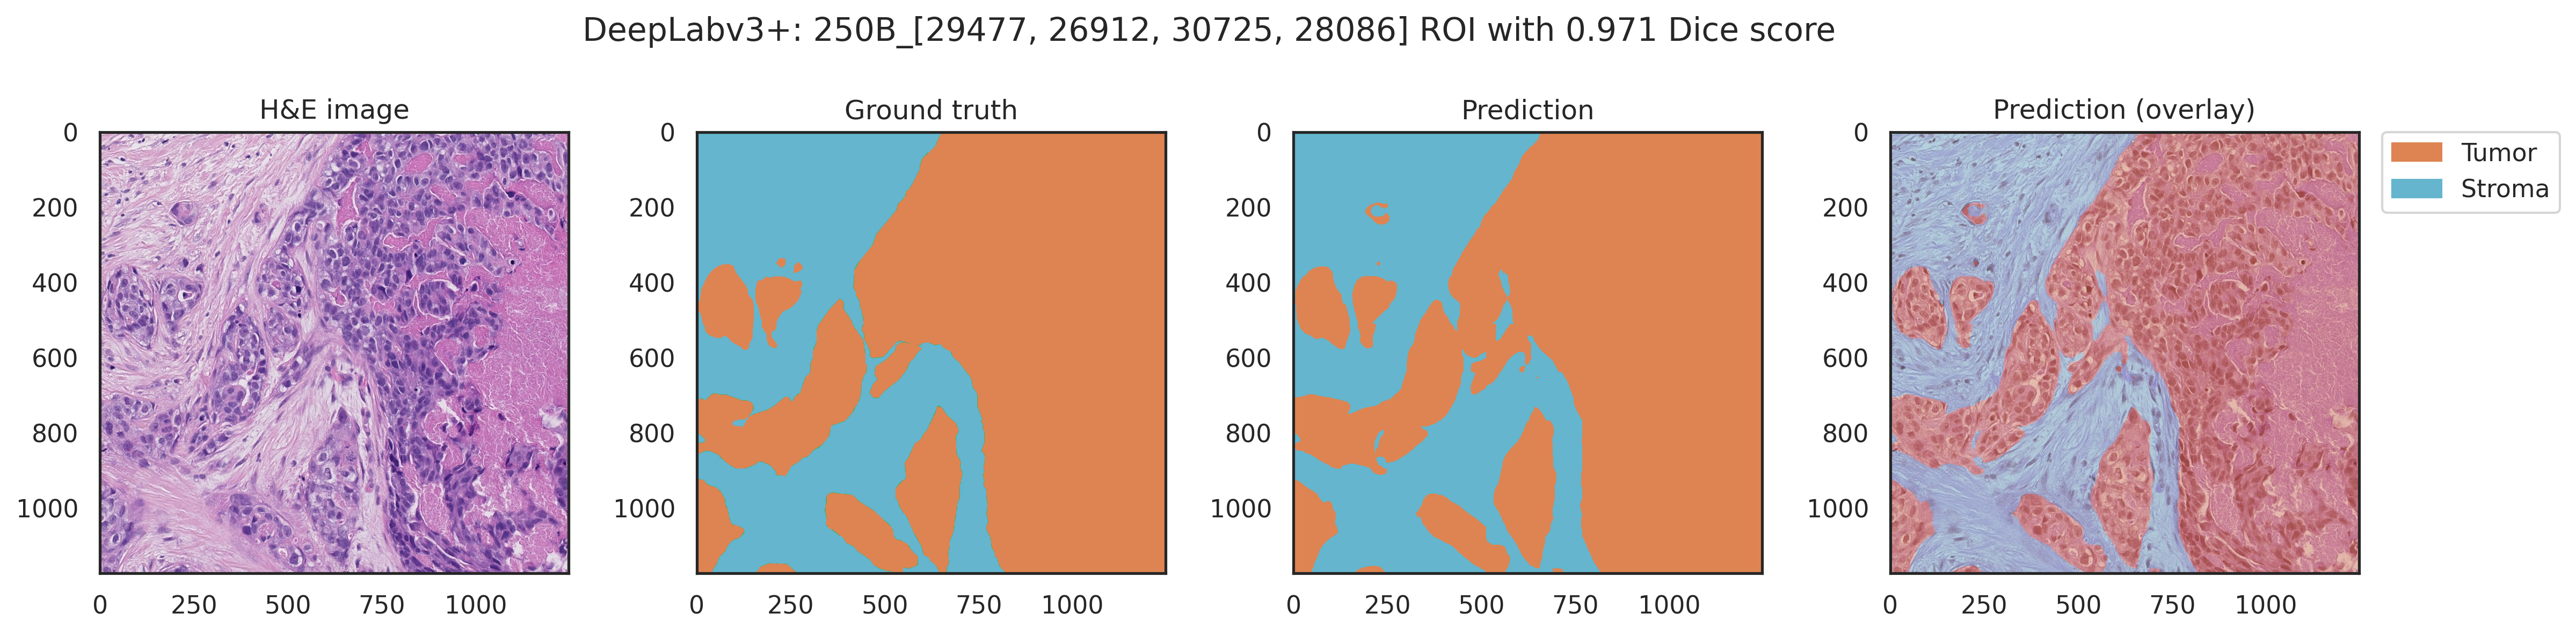
\includegraphics[width=\linewidth]{figures/tissue/deeplabv3+_dice_s_250B_[29477,_26912,_30725,_28086]_check.png}
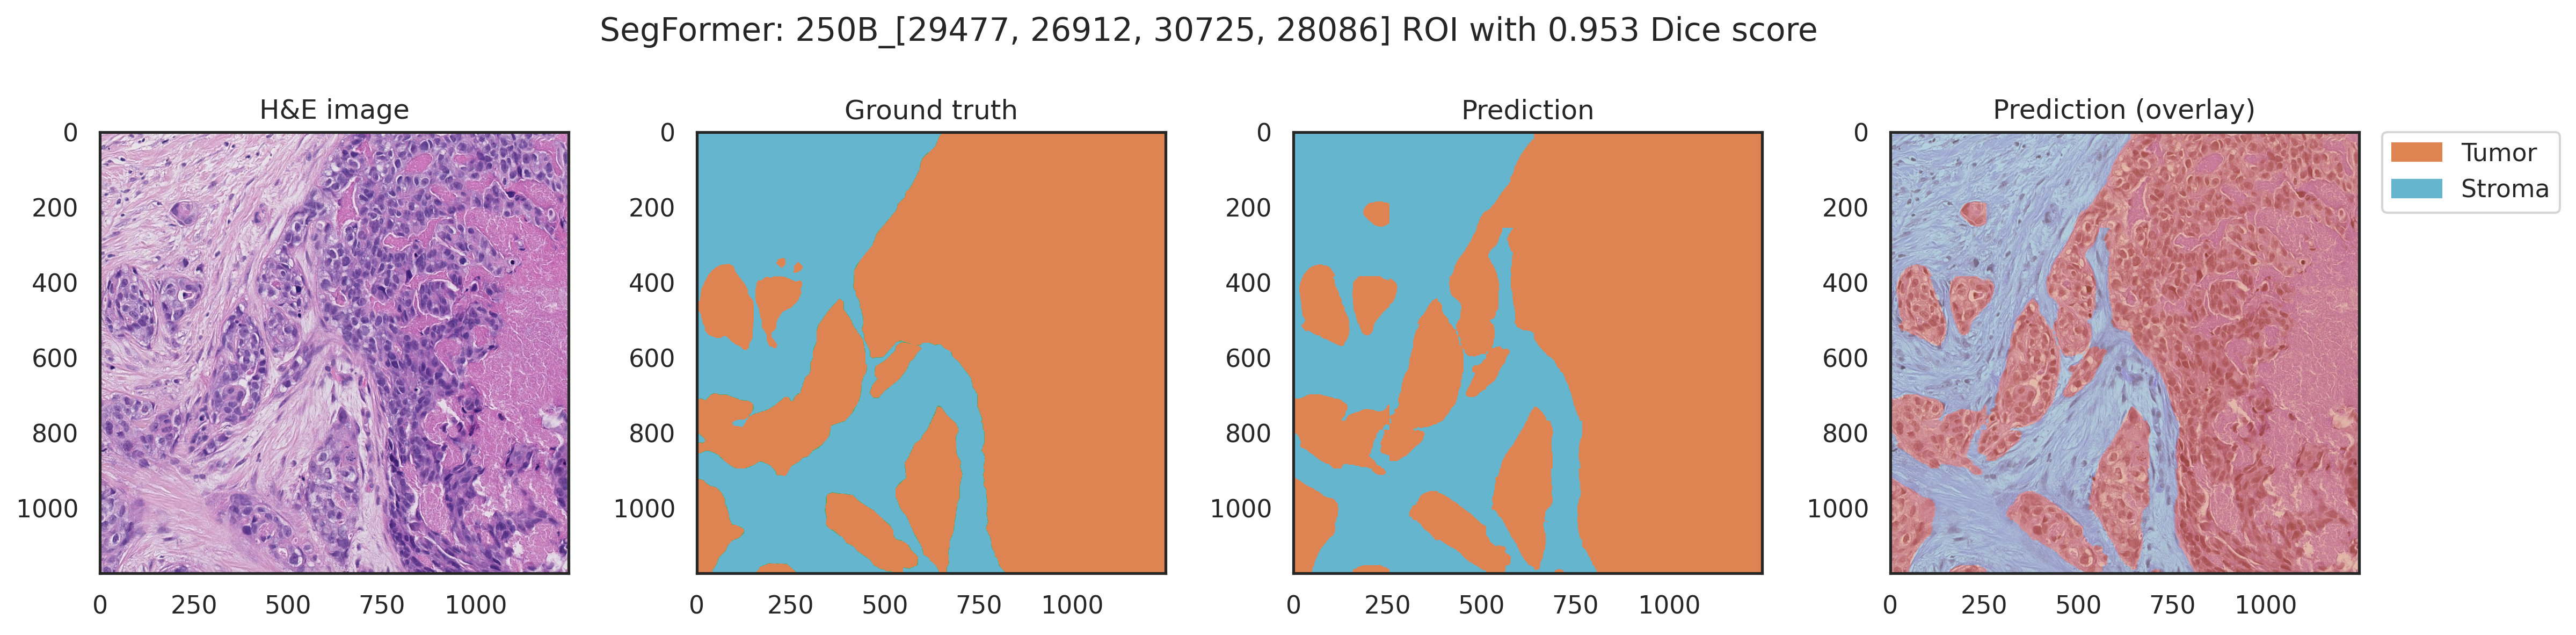
\includegraphics[width=\linewidth]{figures/tissue/segformer_dice_s_250B_[29477,_26912,_30725,_28086]_check.png}
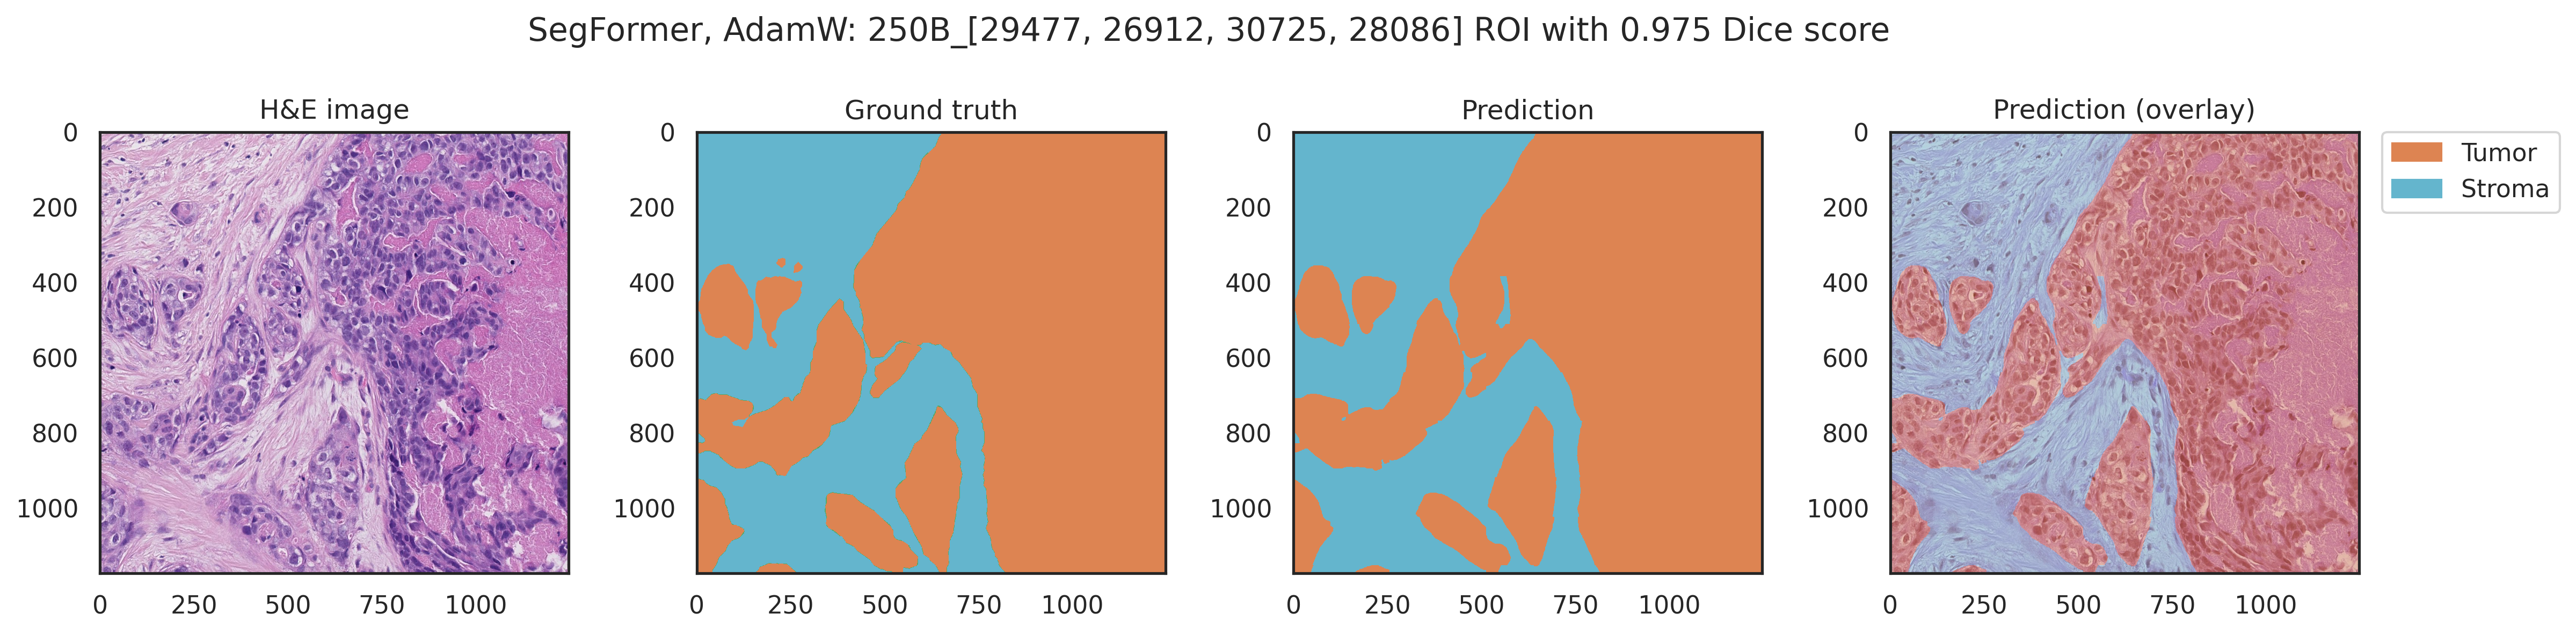
\includegraphics[width=\linewidth]{figures/tissue/segformer,_adamw_dice_s_250B_[29477,_26912,_30725,_28086]_check.png}

\caption{JB ROI segmentation result.}
\label{fig:s_250B_2}
\end{figure}

\begin{figure}[H]
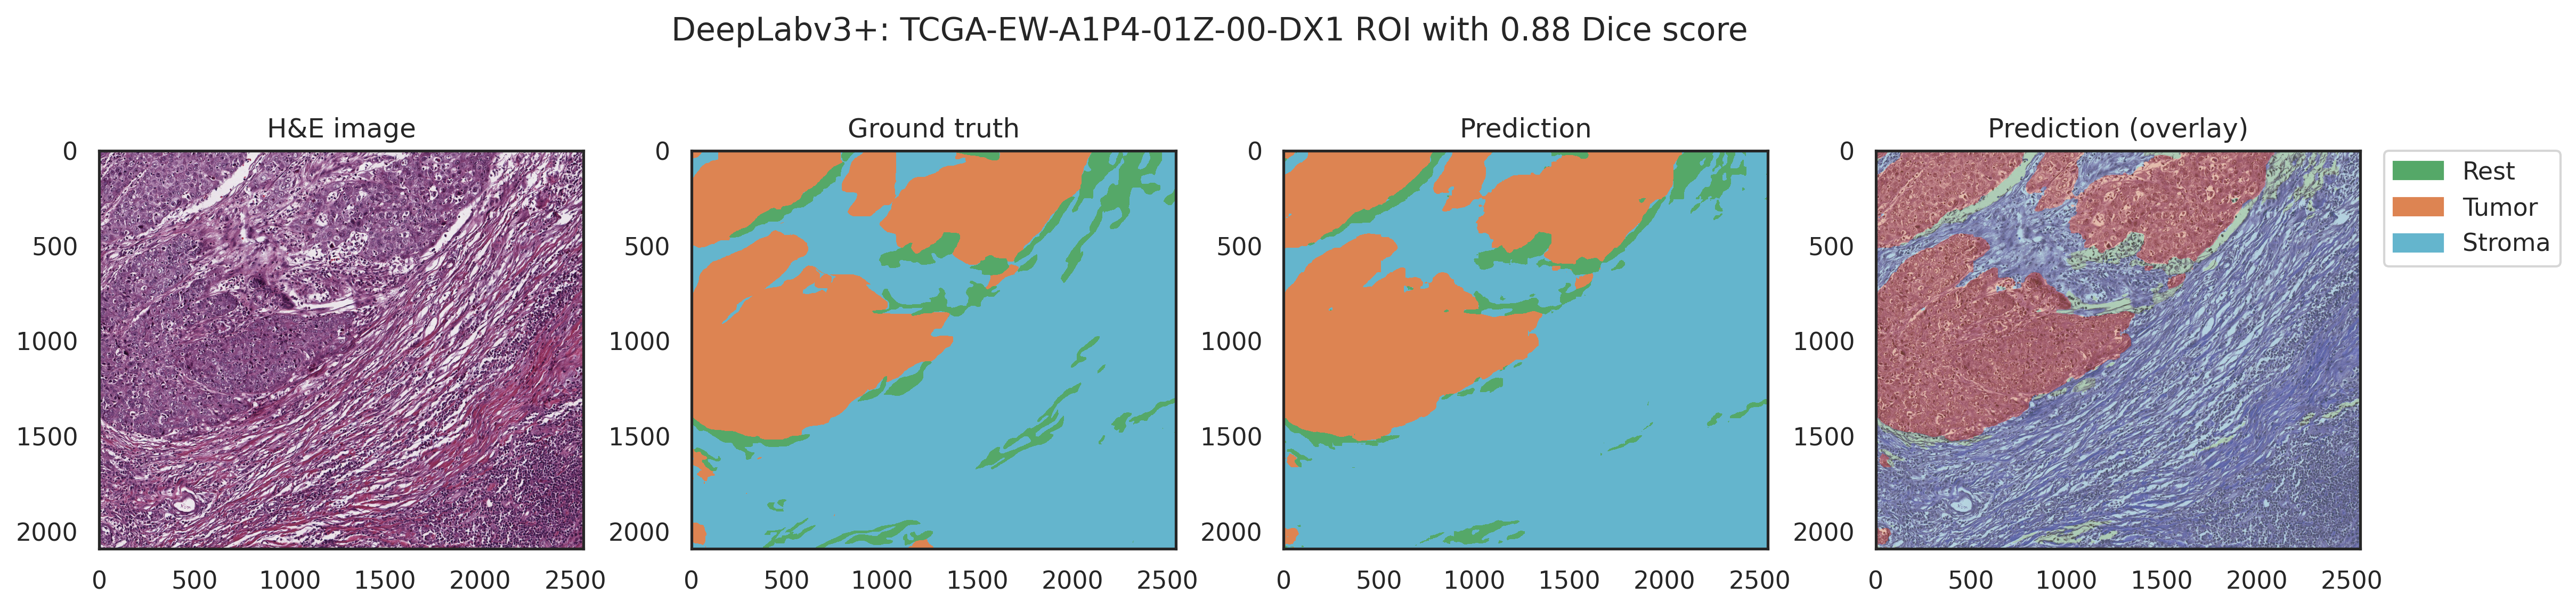
\includegraphics[width=\linewidth]{figures/tissue/deeplabv3+_dice_tcga_TCGA-EW-A1P4-01Z-00-DX13E9AE553-83D4-4B09-AB7F-D096BCE3BC4D_[8630,_17717,_11173,_19809]_check.png}
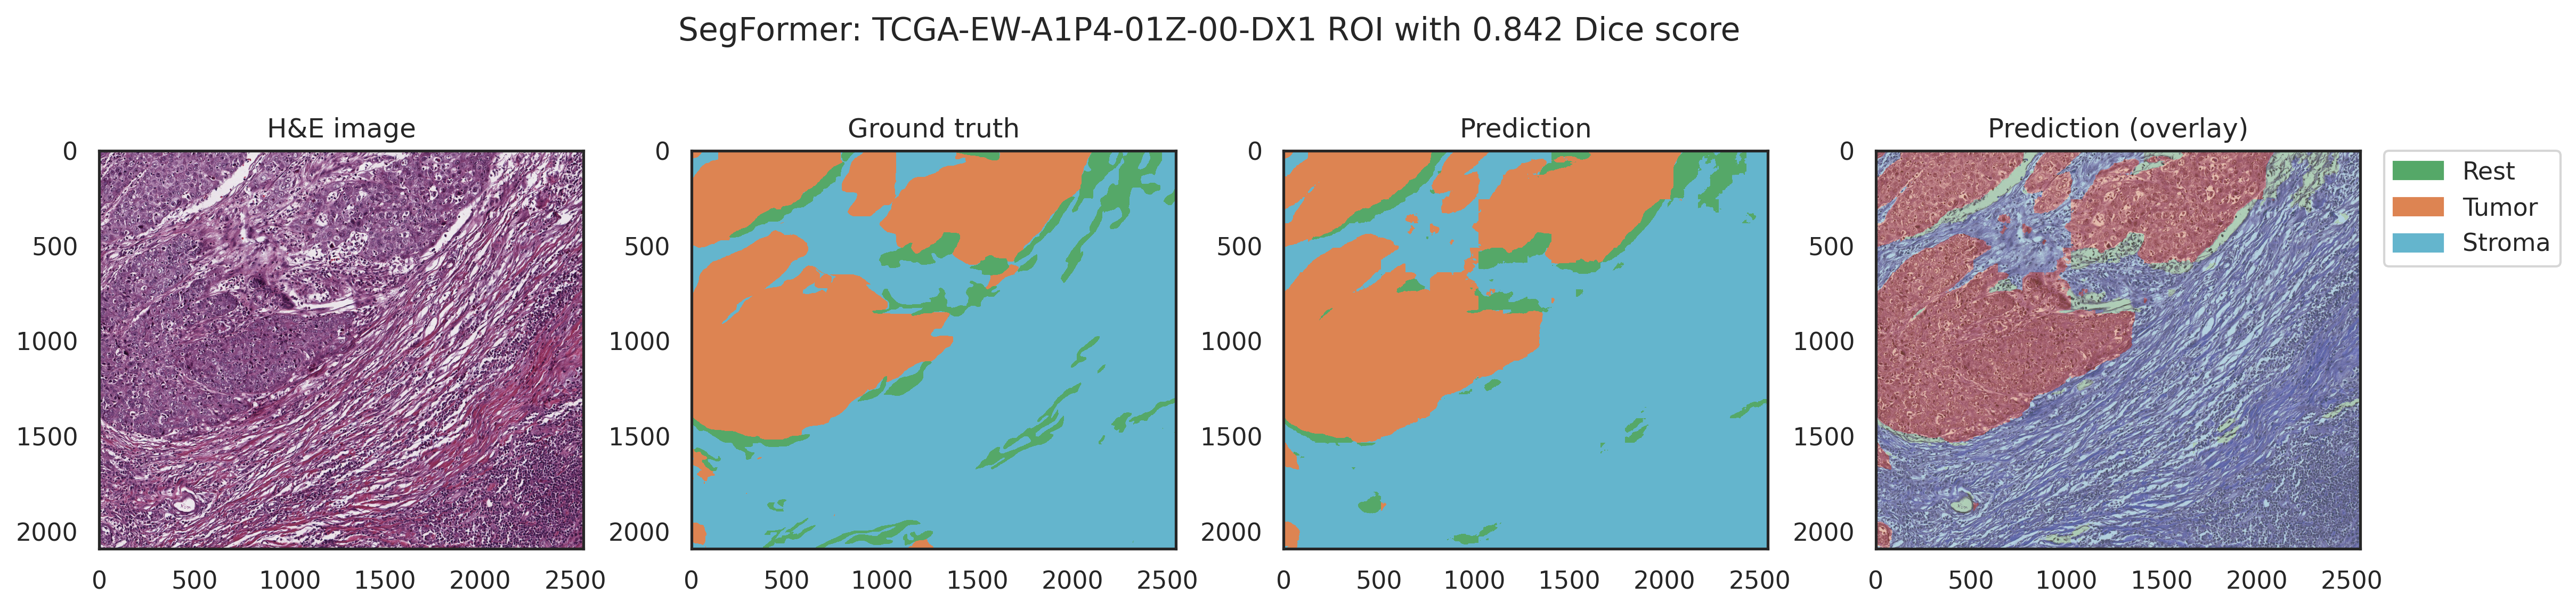
\includegraphics[width=\linewidth]{figures/tissue/segformer_dice_tcga_TCGA-EW-A1P4-01Z-00-DX13E9AE553-83D4-4B09-AB7F-D096BCE3BC4D_[8630,_17717,_11173,_19809]_check.png}
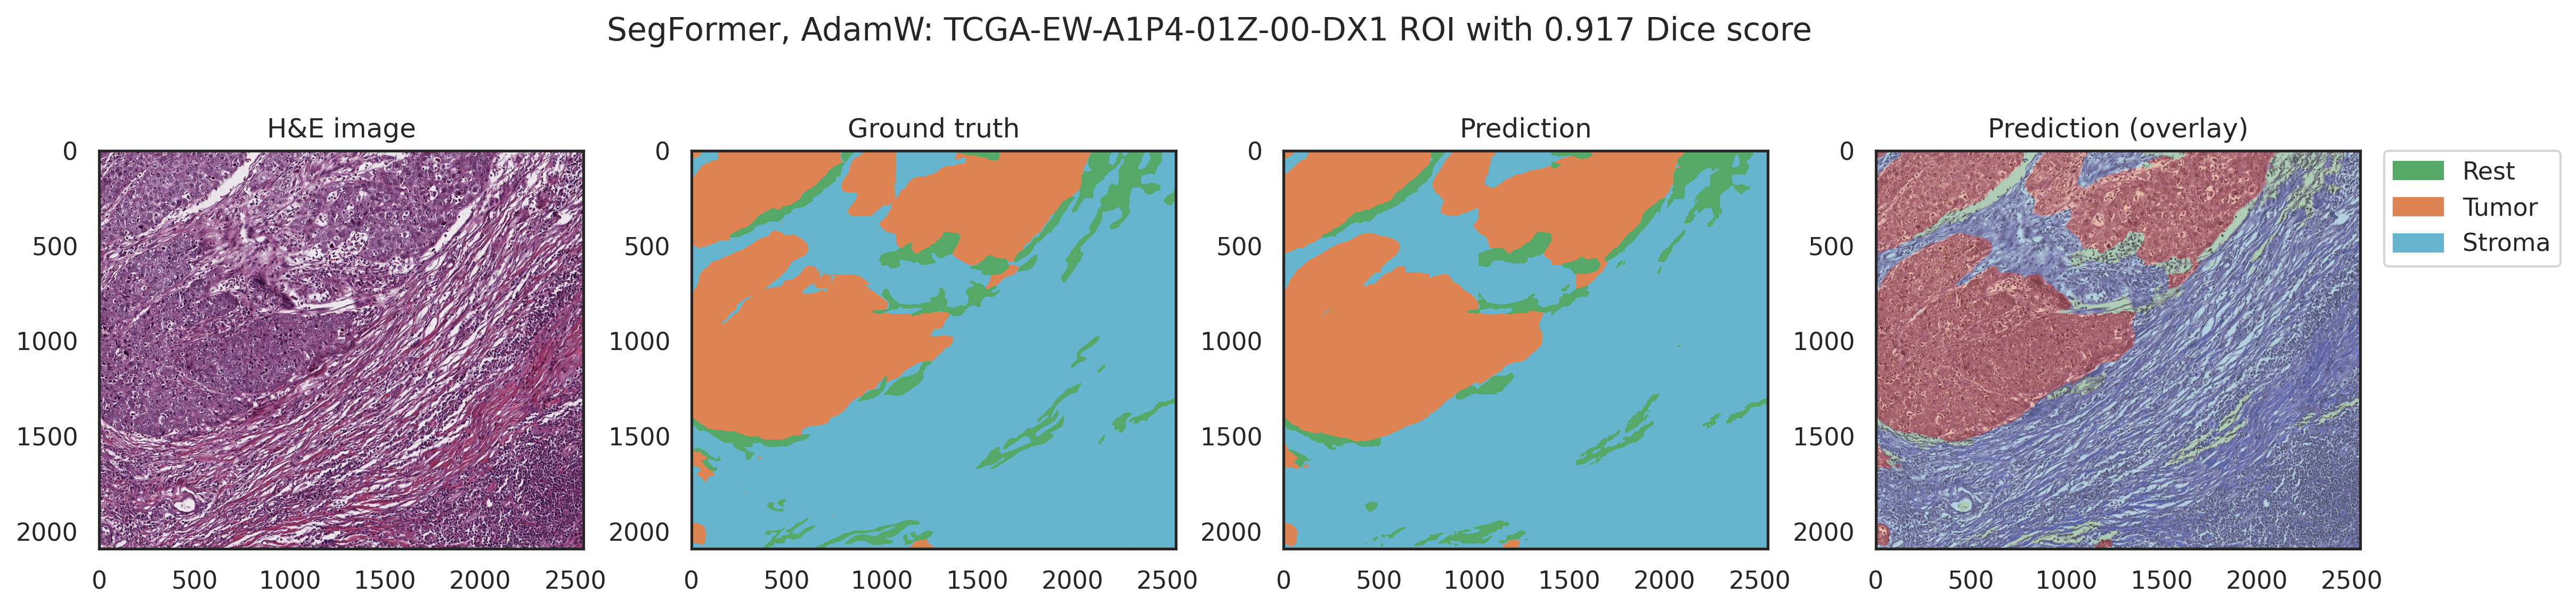
\includegraphics[width=\linewidth]{figures/tissue/segformer,_adamw_dice_tcga_TCGA-EW-A1P4-01Z-00-DX13E9AE553-83D4-4B09-AB7F-D096BCE3BC4D_[8630,_17717,_11173,_19809]_check.png}

\caption{TCGA ROI segmentation result.}
\label{fig:TCGA-EW-A1P4}
\end{figure}



\section{TILs Segmentation}

\begin{figure}[h!]
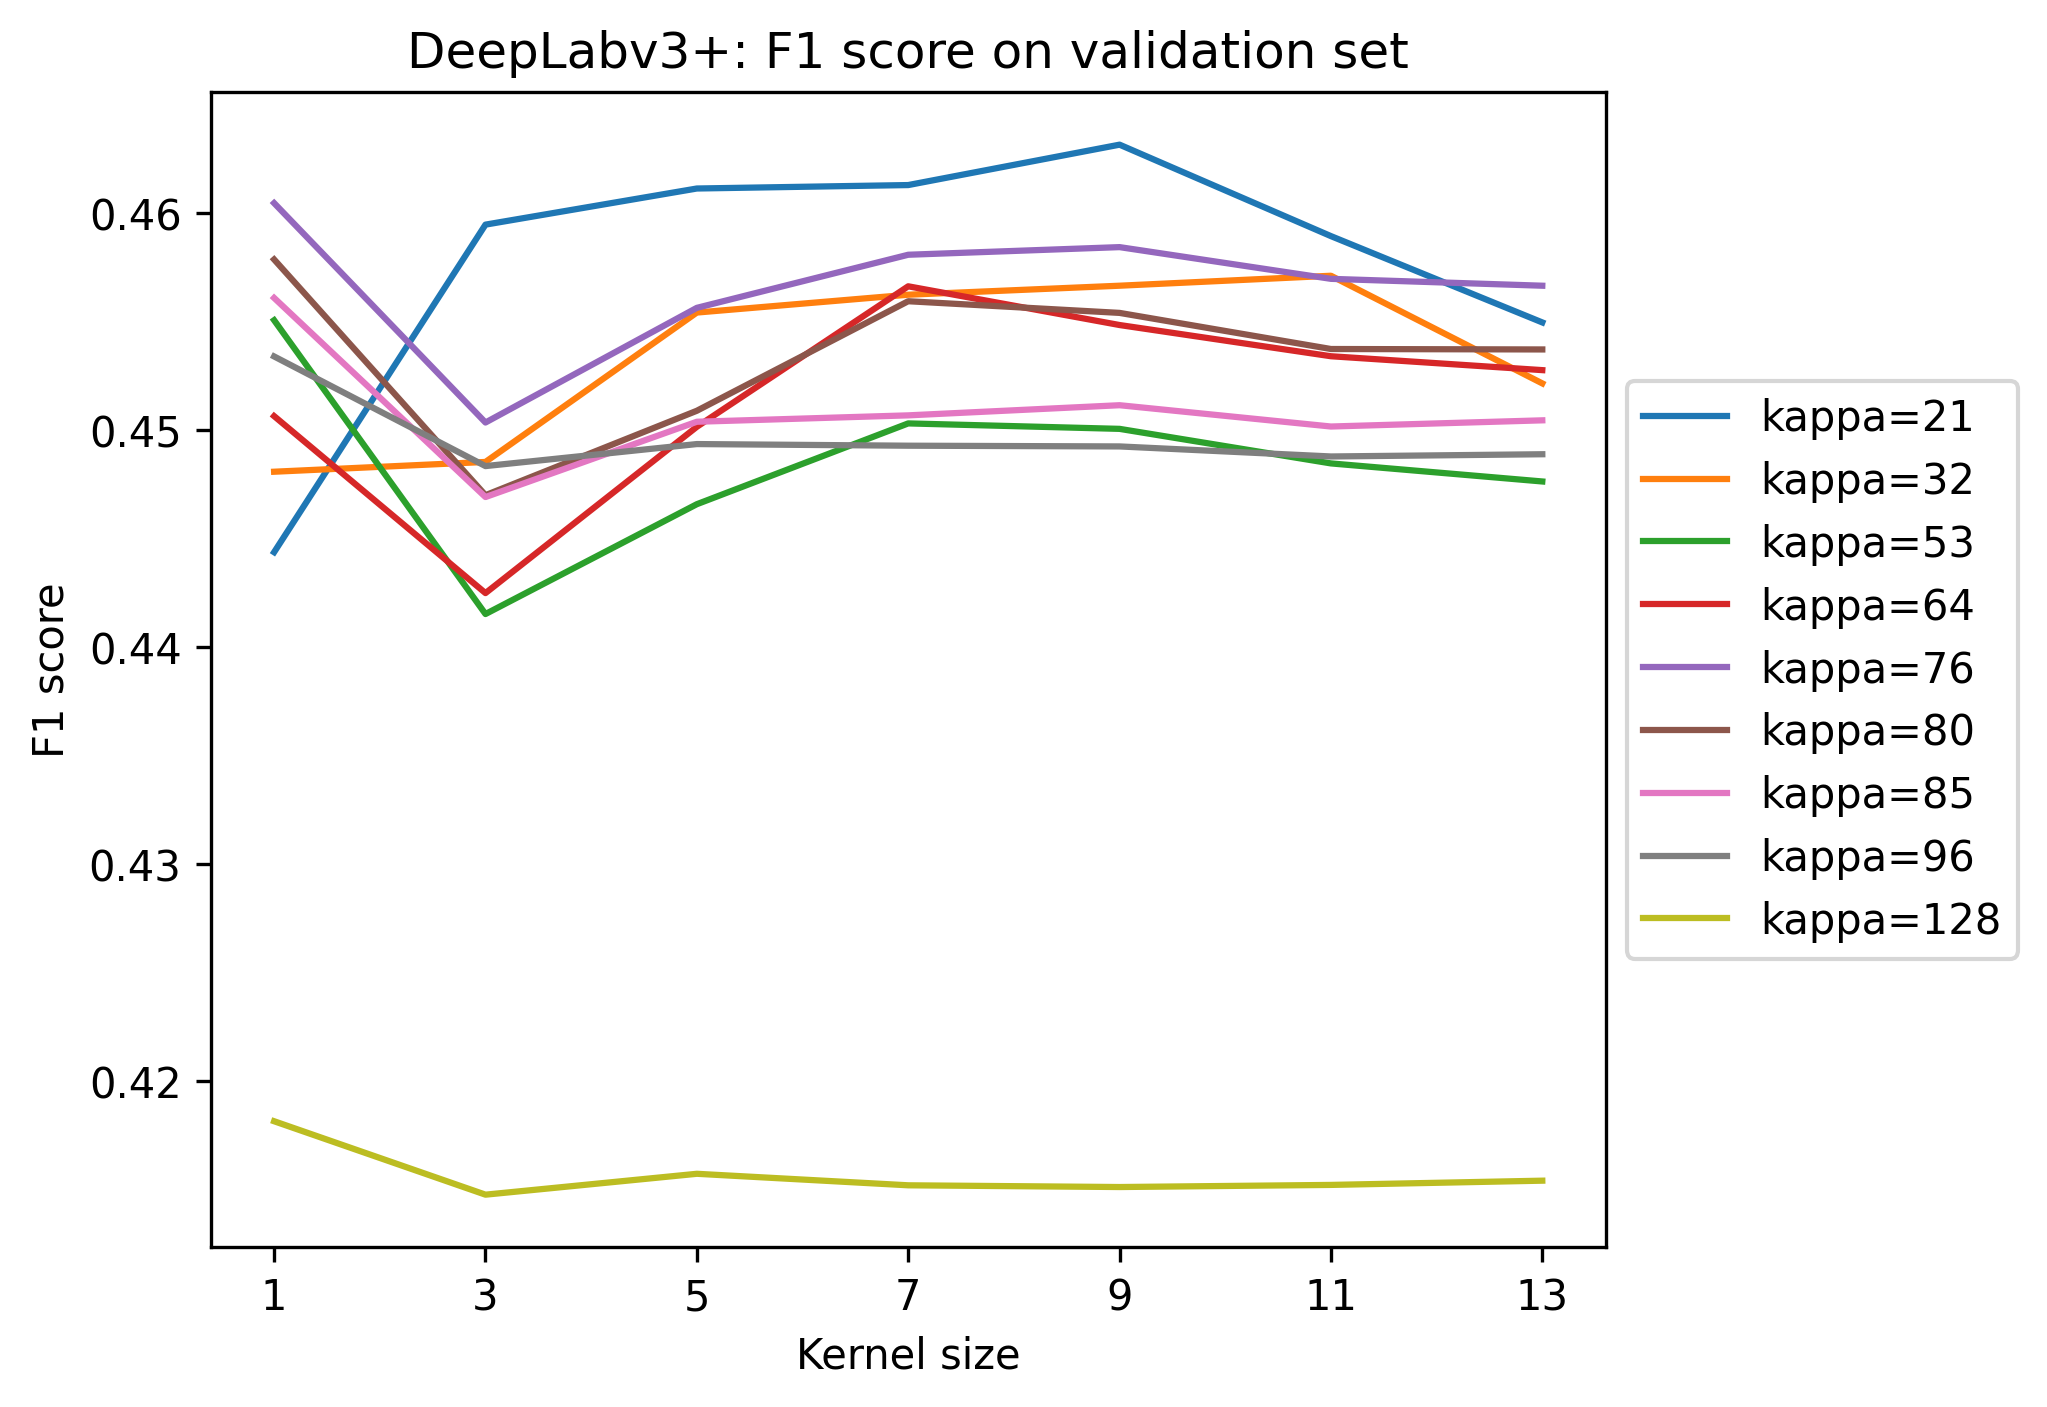
\includegraphics[width=.5\linewidth]{figures/tils/deeplabv3+_f1_kappas_kernels_plot.png}
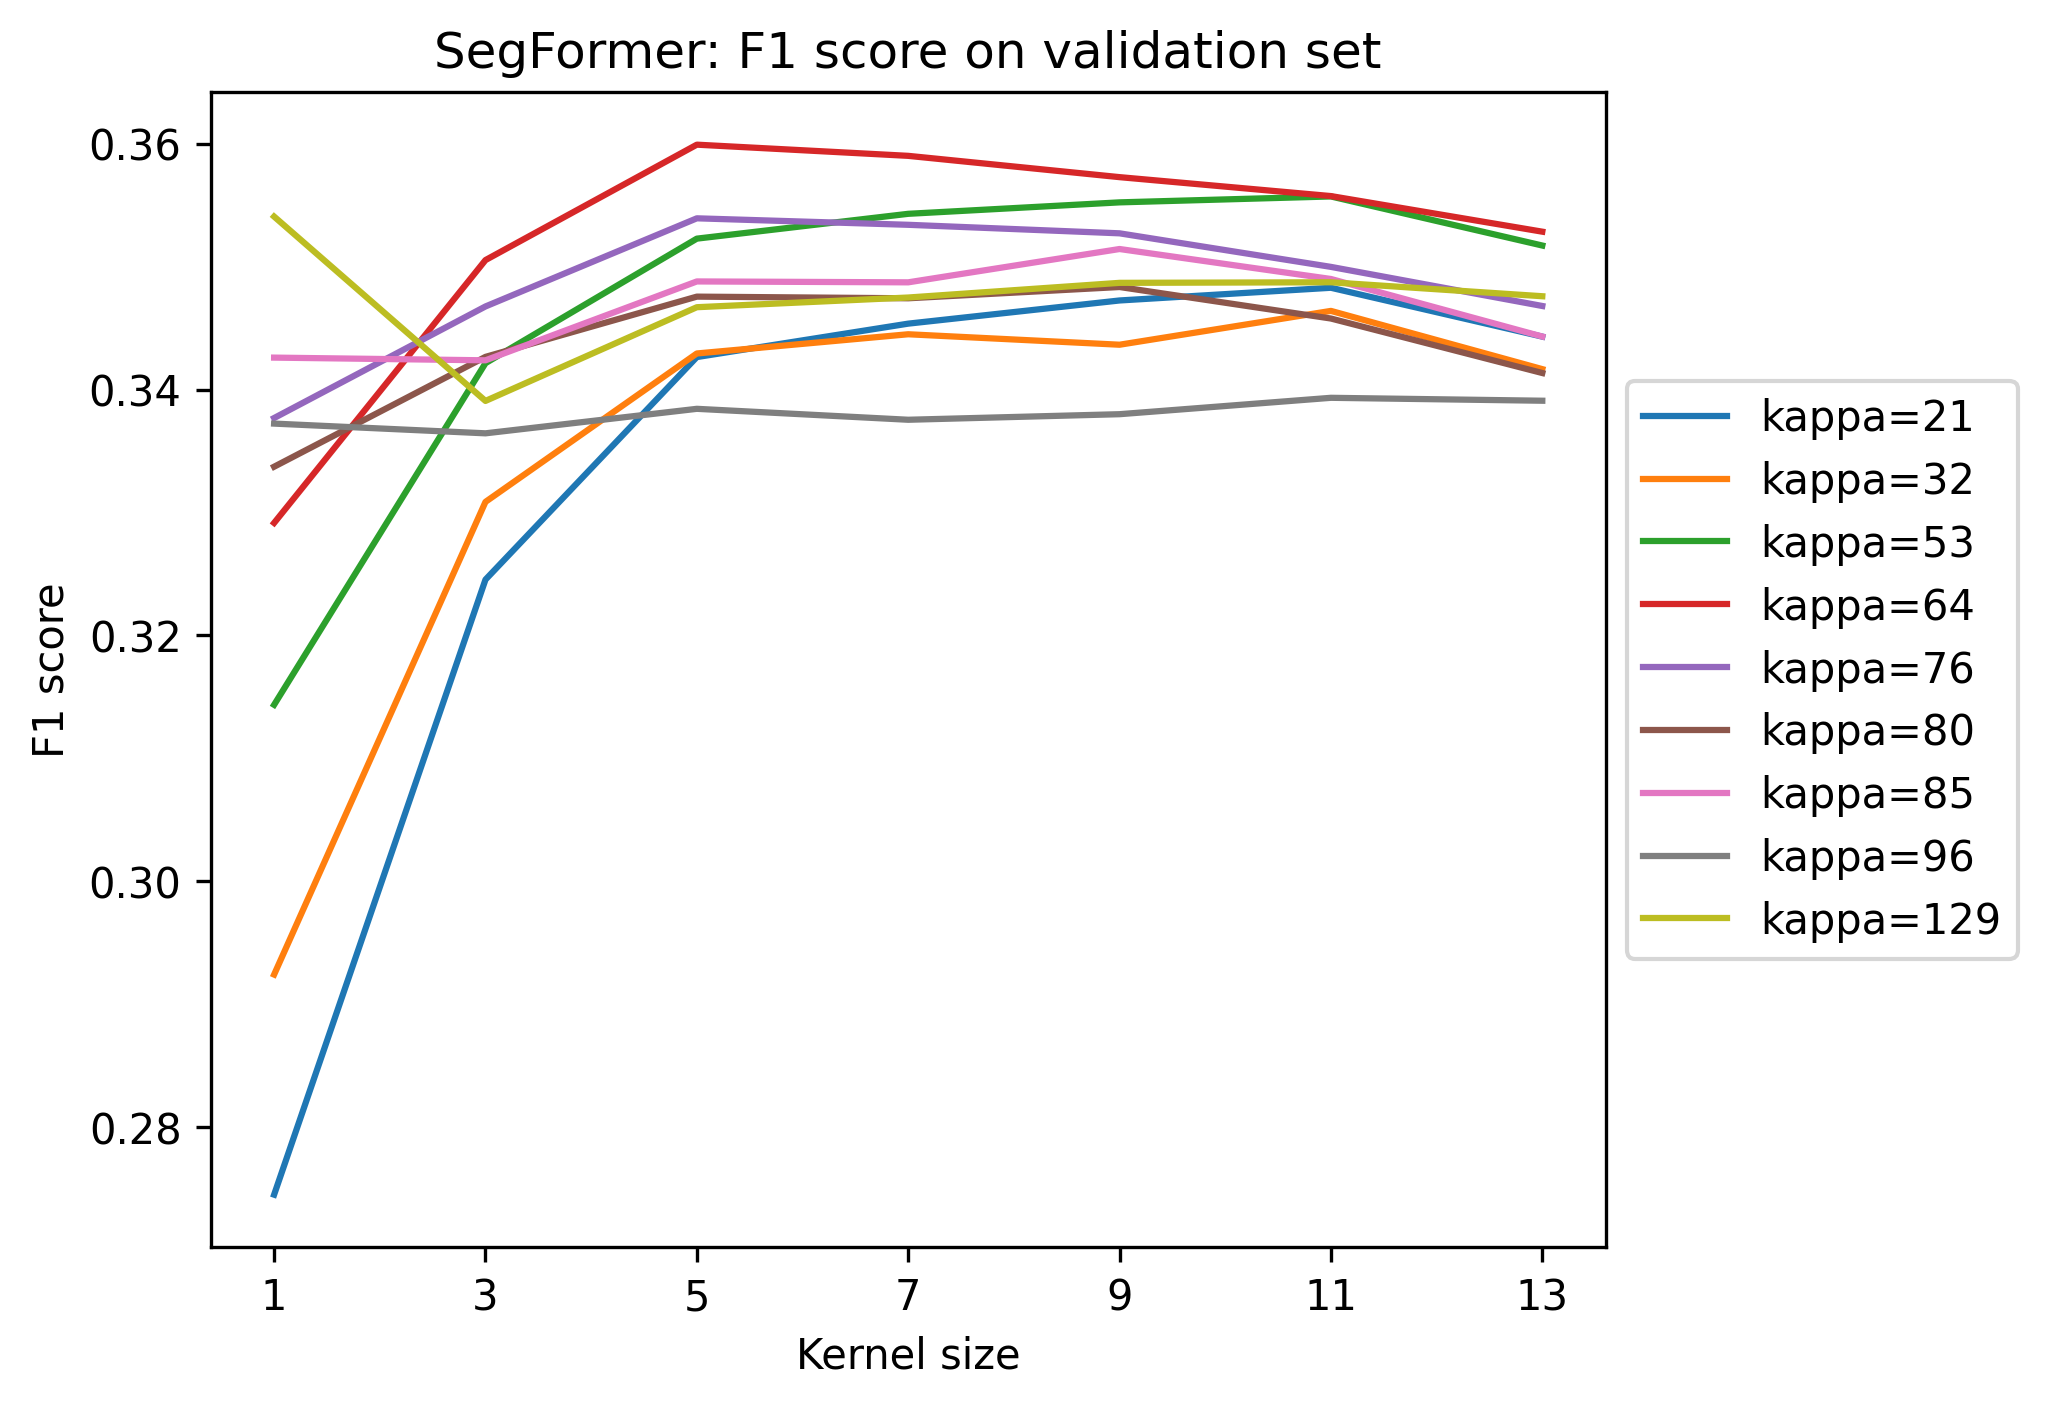
\includegraphics[width=.5\linewidth]{figures/tils/segformer_f1_kappas_kernels_plot.png}

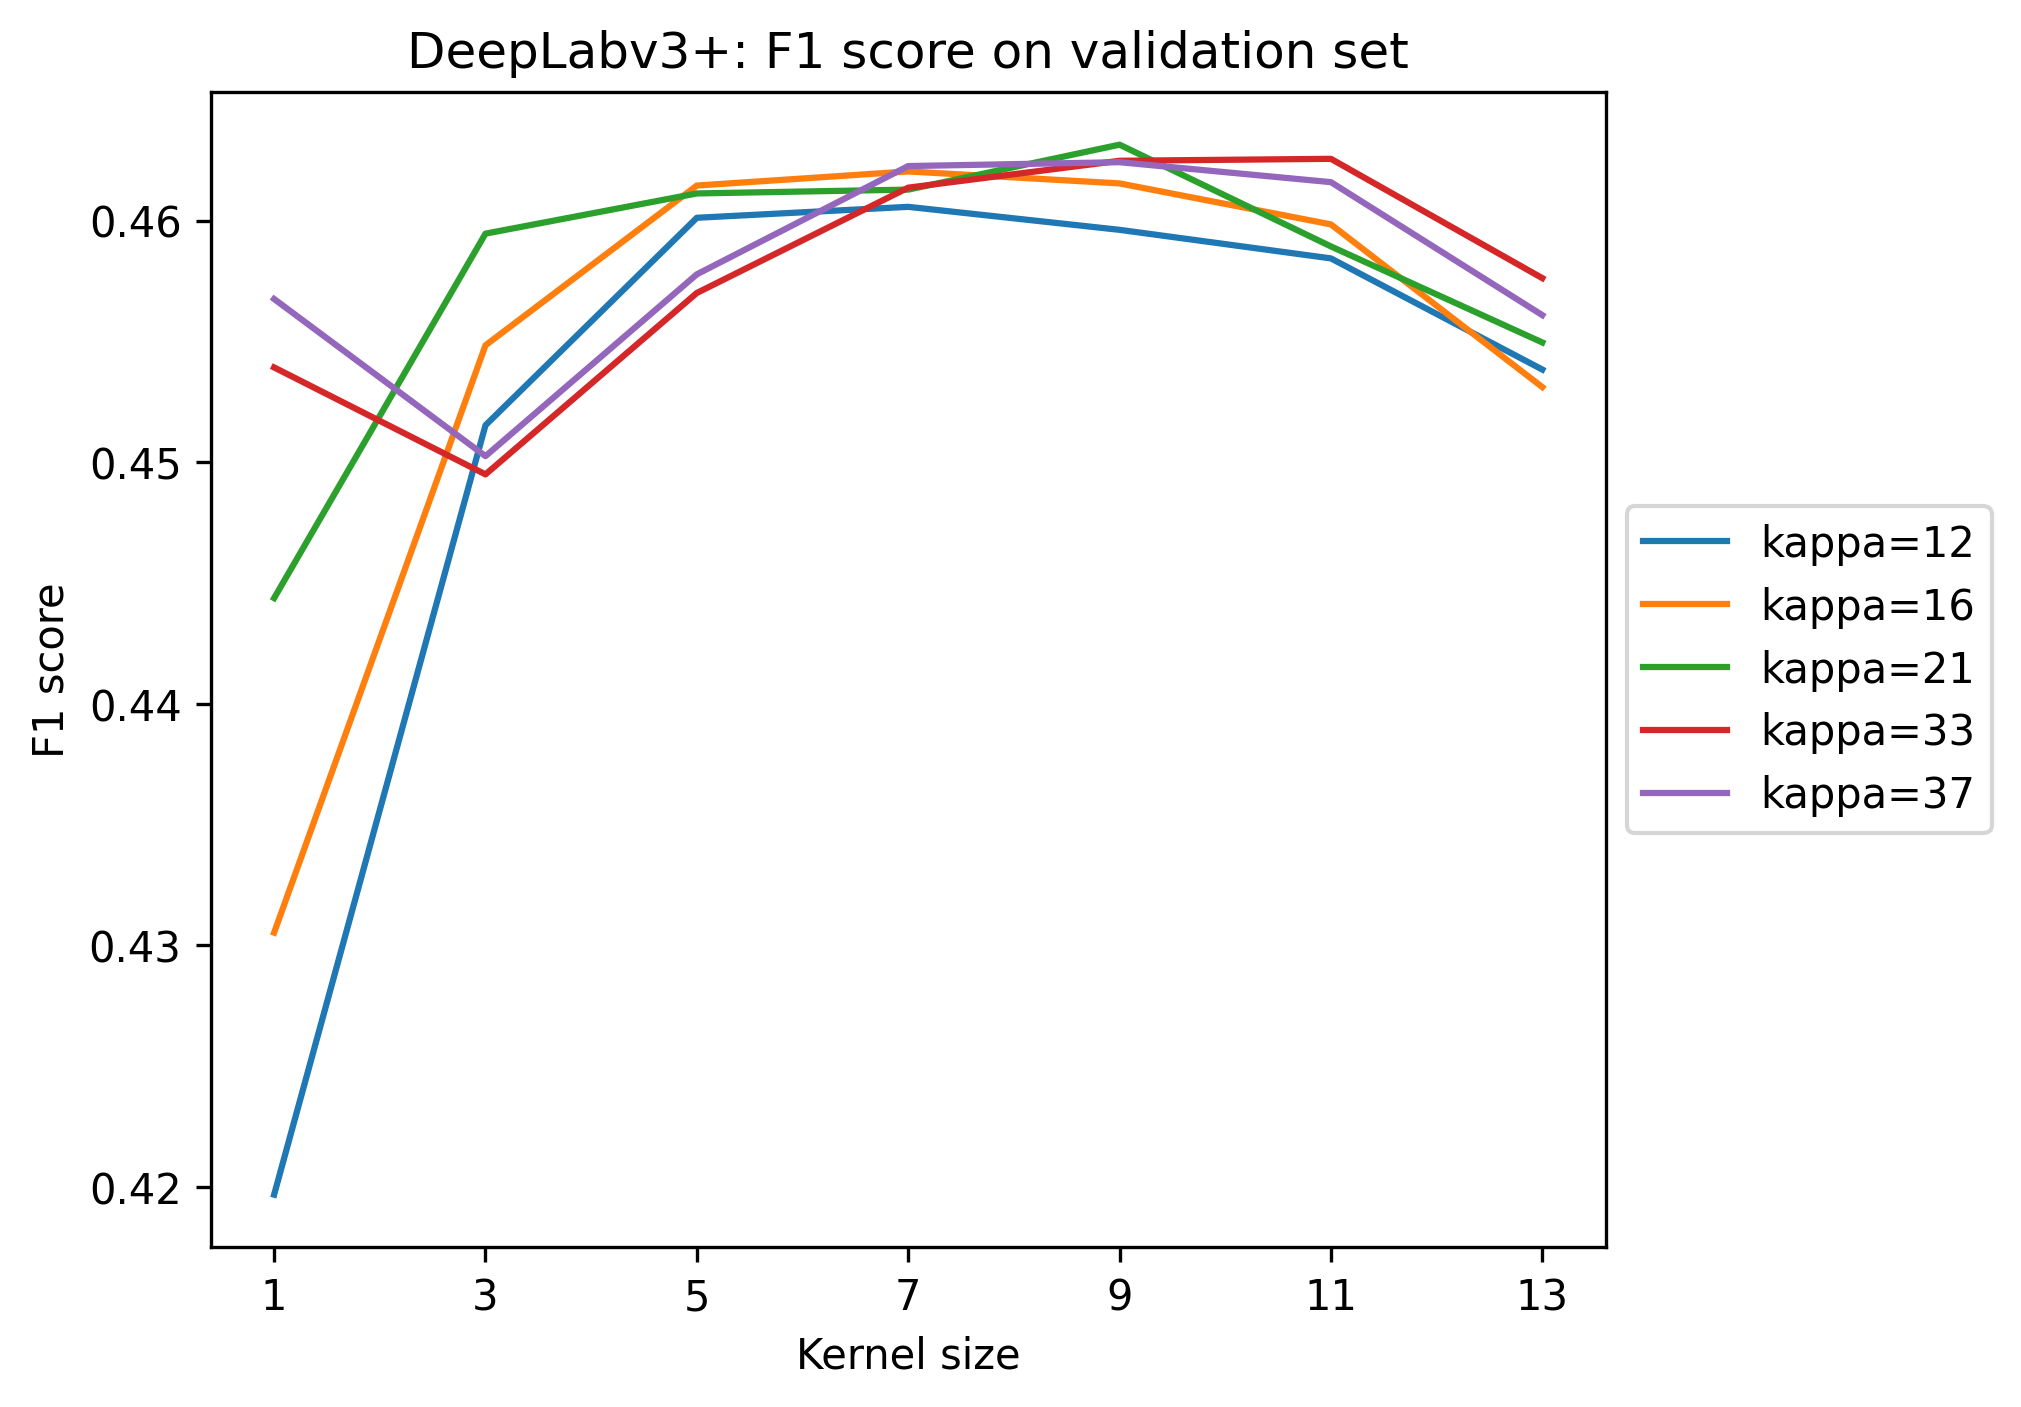
\includegraphics[width=.5\linewidth]{figures/tils/deeplabv3+_f1_kappas_kernels_plot_zooomed.png}
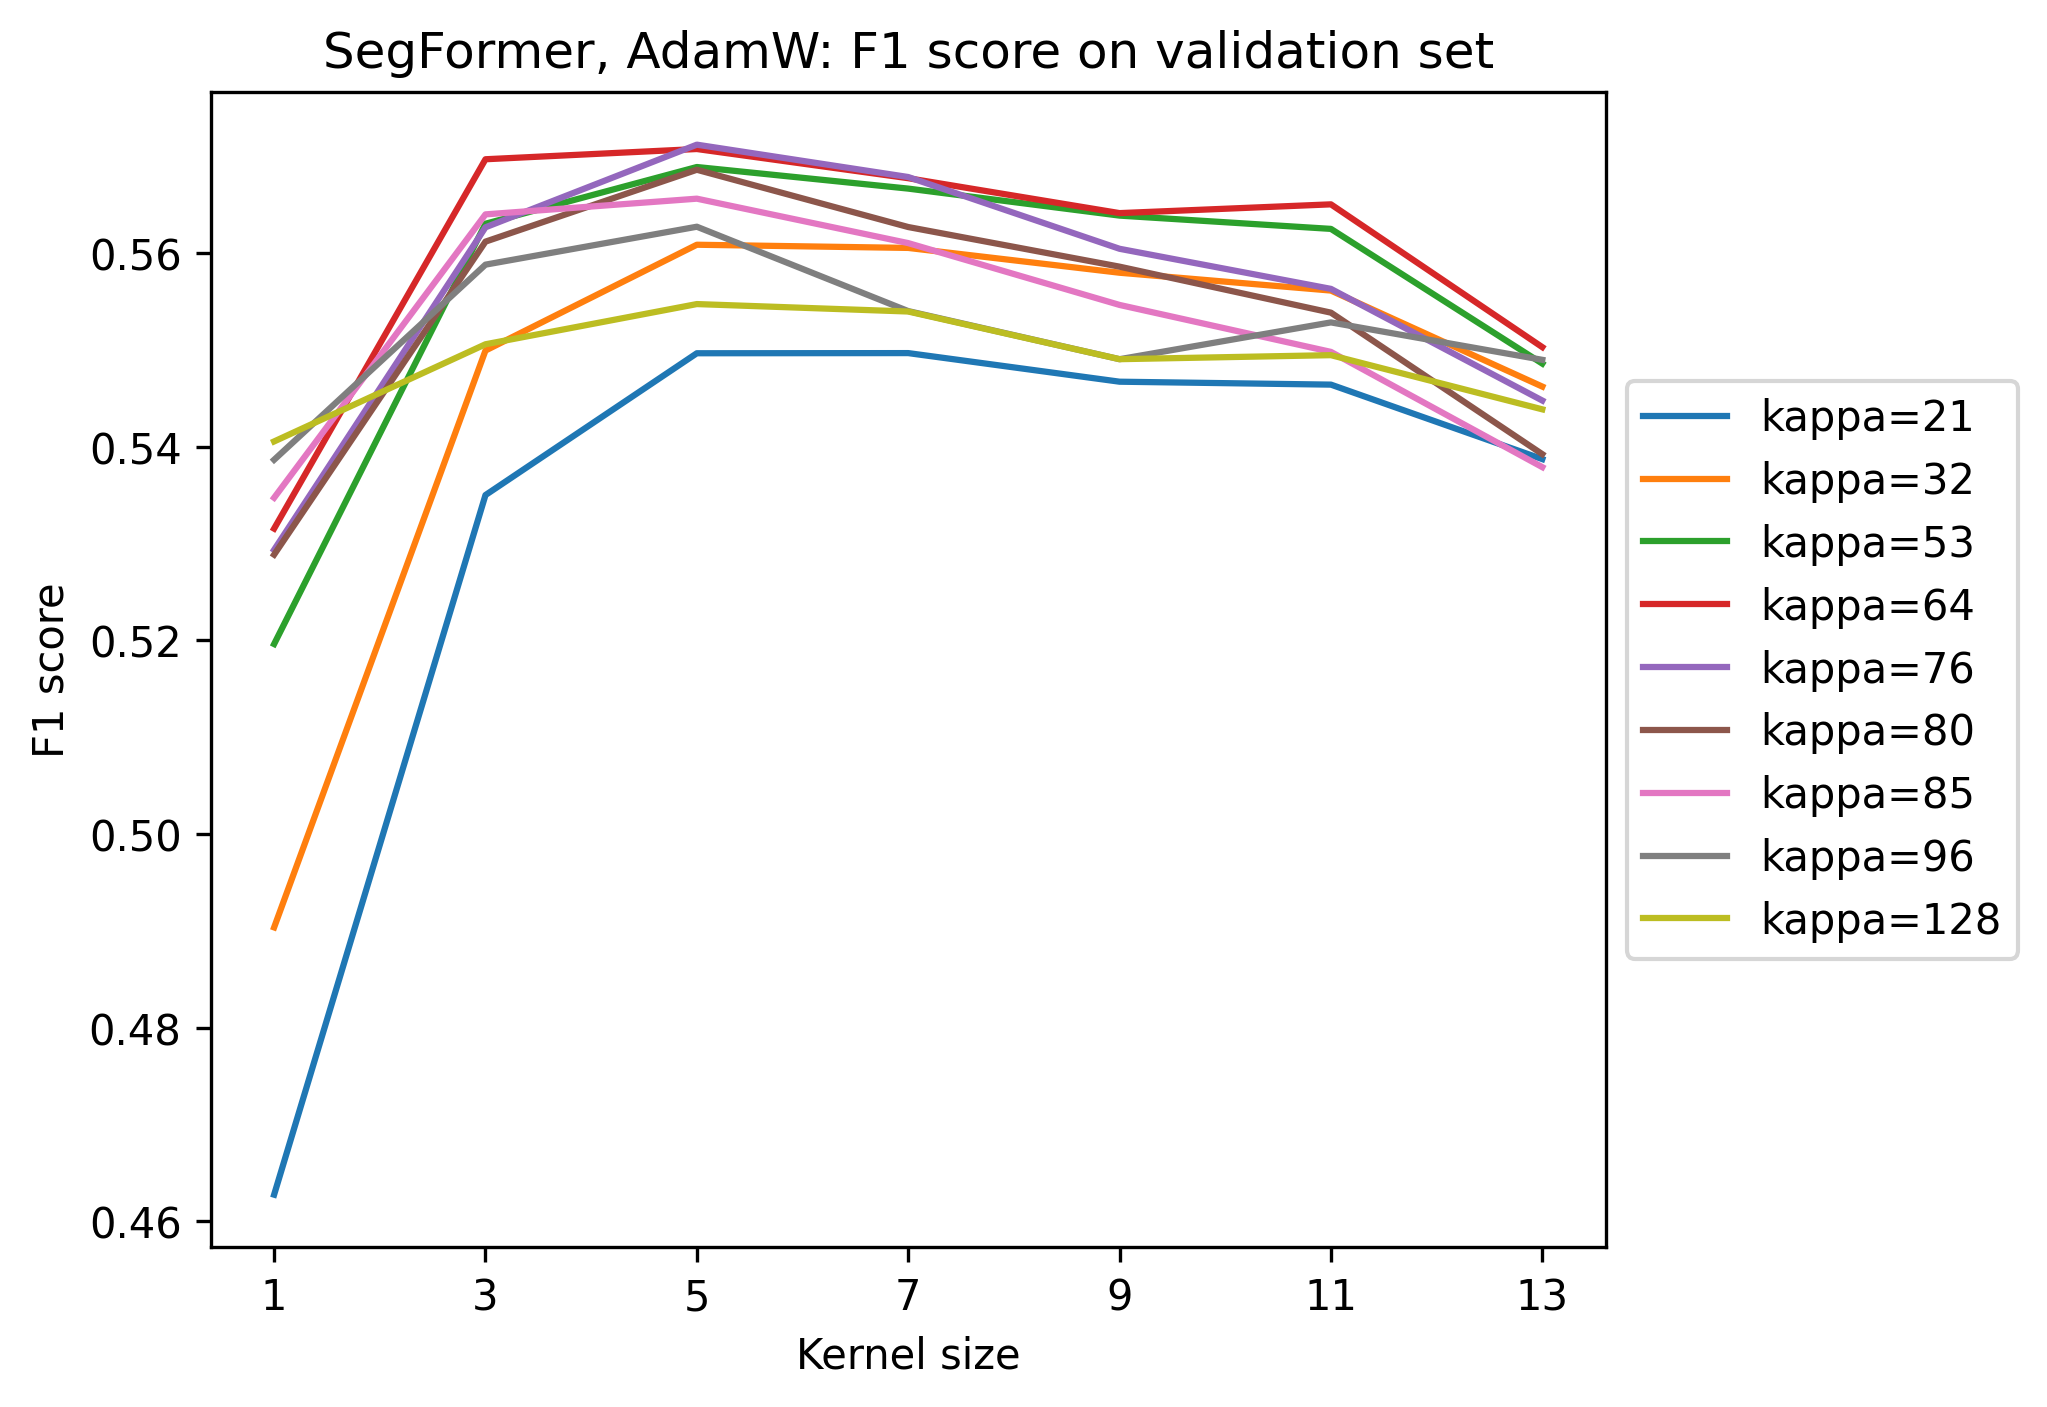
\includegraphics[width=.5\linewidth]{figures/tils/segformer,_adamw_f1_kappas_kernels_plot.png}

\caption{EXAMPLES for TILs prediction models. A lot of test comming up here.}
\label{fig:figure3}

\end{figure}

\begin{figure}[h!]
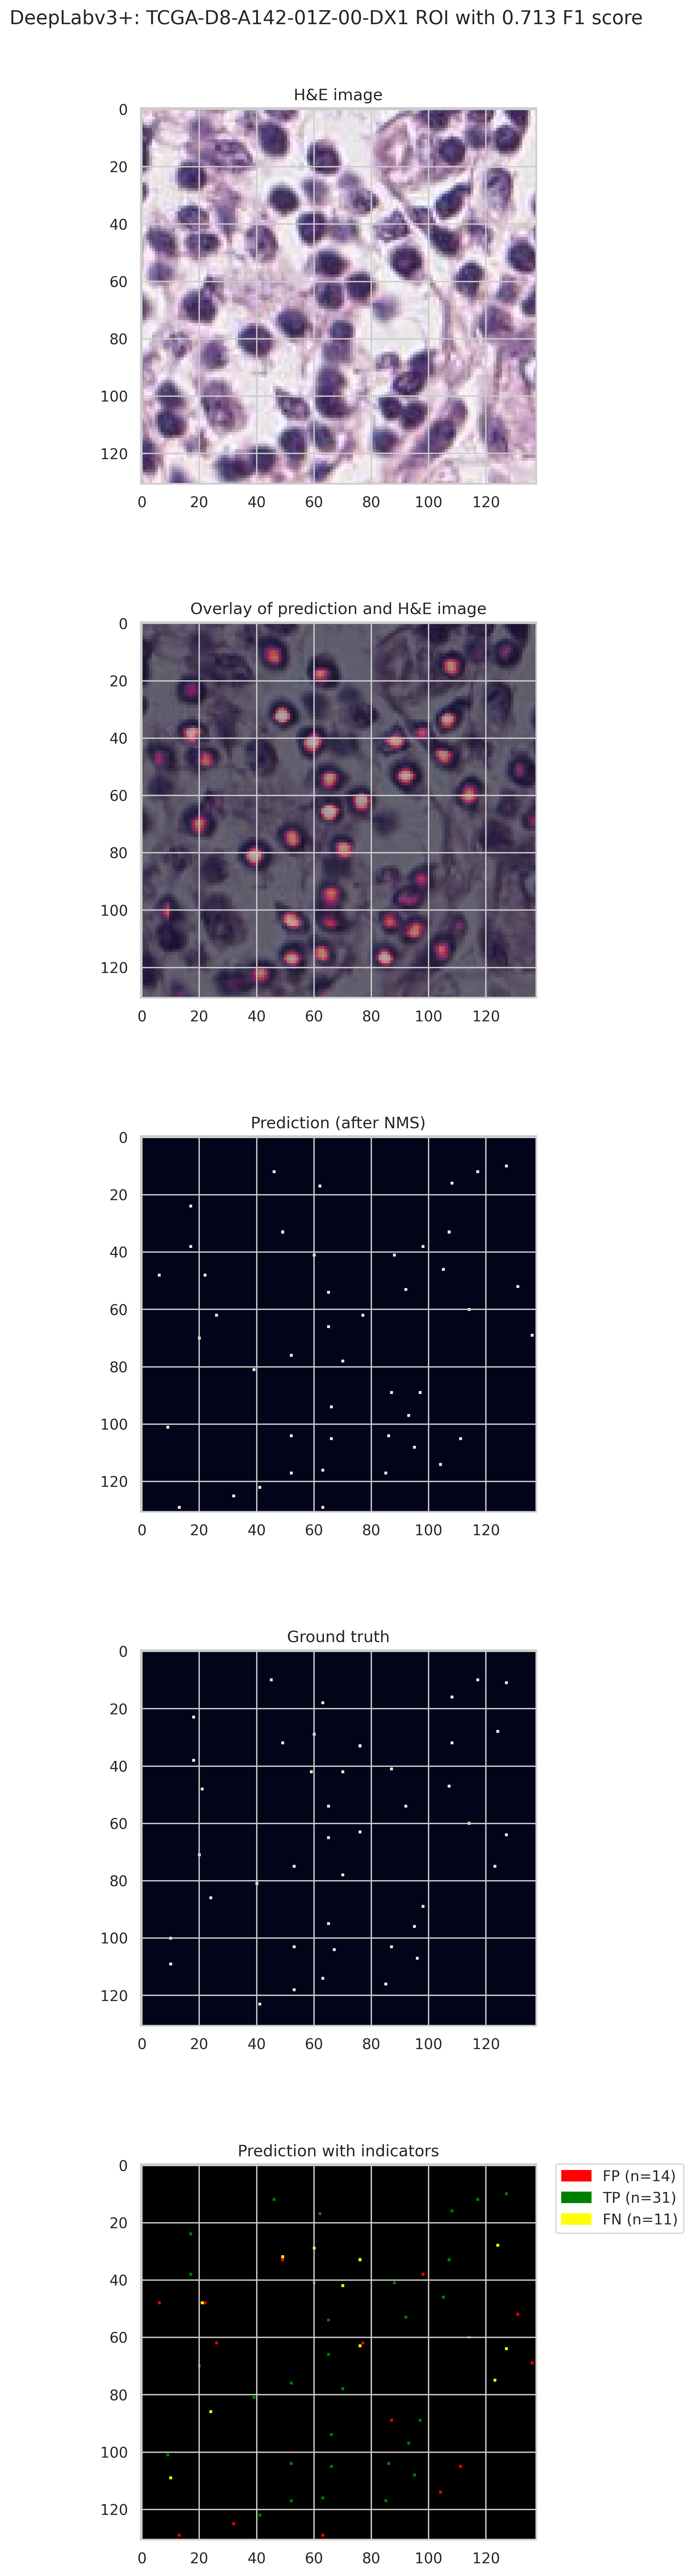
\includegraphics[width=.305\textwidth]{figures/tils/TCGA-D8-A142-01Z-00-DX1_F1_deeplabv3+_adj.png}
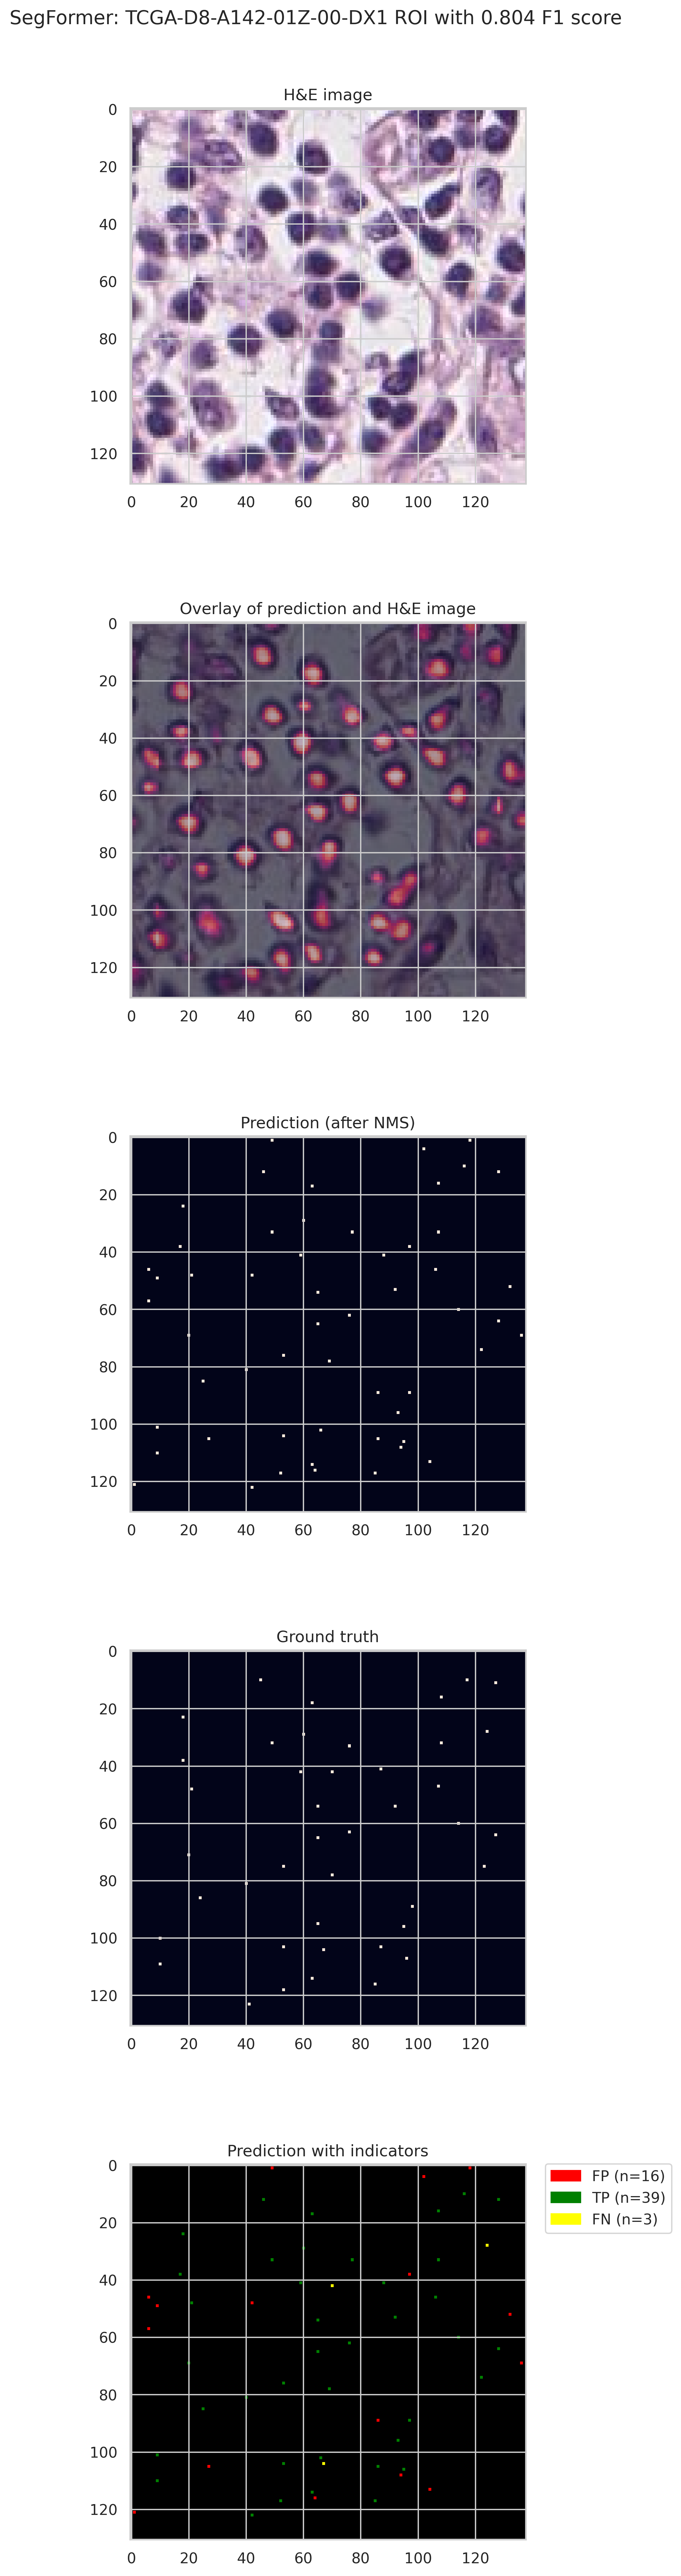
\includegraphics[width=.3\textwidth]{figures/tils/TCGA-D8-A142-01Z-00-DX1_F1_segformer_adj.png}
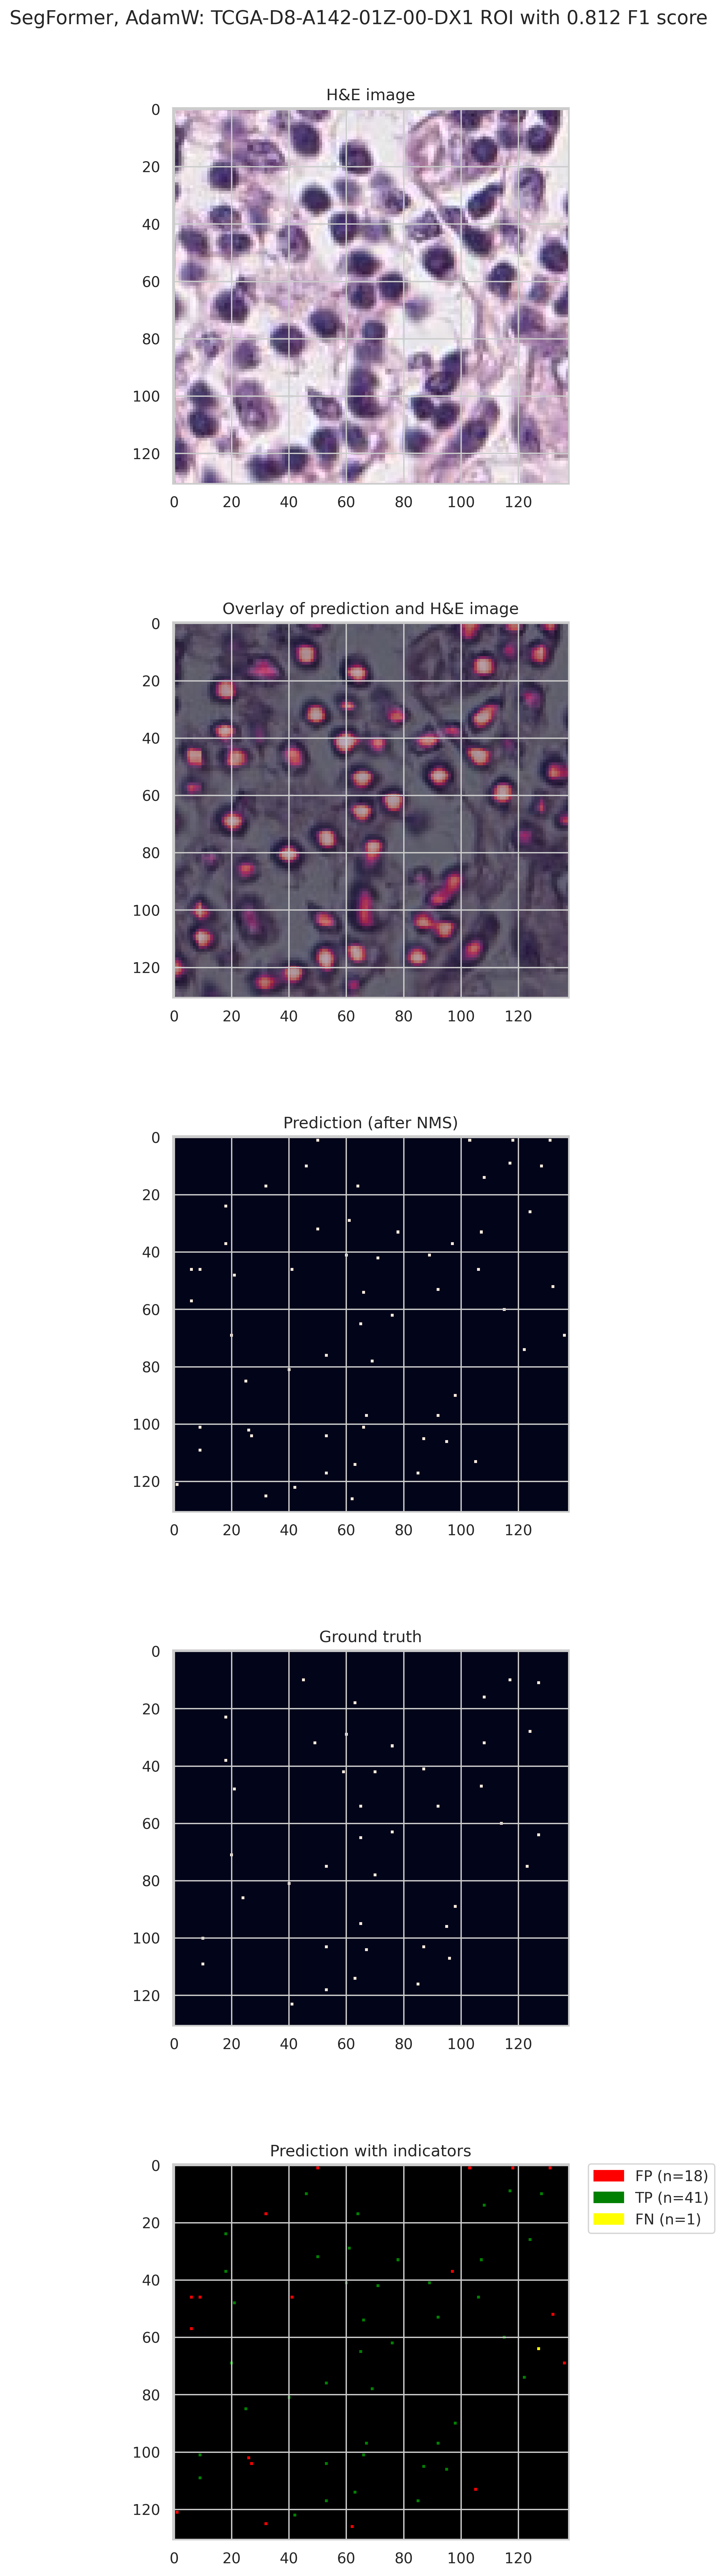
\includegraphics[width=.319\textwidth]{figures/tils/TCGA-D8-A142-01Z-00-DX1_F1_segformer,_adamw_adj.png}
\caption{EXAMPLES for TILs prediction models. A lot of test comming up here.}
\label{fig:figure3}

\end{figure}